\documentclass[12pt,a4paper]{article}\usepackage[]{graphicx}\usepackage[]{color}
%% maxwidth is the original width if it is less than linewidth
%% otherwise use linewidth (to make sure the graphics do not exceed the margin)
\makeatletter
\def\maxwidth{ %
  \ifdim\Gin@nat@width>\linewidth
    \linewidth
  \else
    \Gin@nat@width
  \fi
}
\makeatother

\definecolor{fgcolor}{rgb}{0.345, 0.345, 0.345}
\newcommand{\hlnum}[1]{\textcolor[rgb]{0.686,0.059,0.569}{#1}}%
\newcommand{\hlstr}[1]{\textcolor[rgb]{0.192,0.494,0.8}{#1}}%
\newcommand{\hlcom}[1]{\textcolor[rgb]{0.678,0.584,0.686}{\textit{#1}}}%
\newcommand{\hlopt}[1]{\textcolor[rgb]{0,0,0}{#1}}%
\newcommand{\hlstd}[1]{\textcolor[rgb]{0.345,0.345,0.345}{#1}}%
\newcommand{\hlkwa}[1]{\textcolor[rgb]{0.161,0.373,0.58}{\textbf{#1}}}%
\newcommand{\hlkwb}[1]{\textcolor[rgb]{0.69,0.353,0.396}{#1}}%
\newcommand{\hlkwc}[1]{\textcolor[rgb]{0.333,0.667,0.333}{#1}}%
\newcommand{\hlkwd}[1]{\textcolor[rgb]{0.737,0.353,0.396}{\textbf{#1}}}%

\usepackage{framed}
\makeatletter
\newenvironment{kframe}{%
 \def\at@end@of@kframe{}%
 \ifinner\ifhmode%
  \def\at@end@of@kframe{\end{minipage}}%
  \begin{minipage}{\columnwidth}%
 \fi\fi%
 \def\FrameCommand##1{\hskip\@totalleftmargin \hskip-\fboxsep
 \colorbox{shadecolor}{##1}\hskip-\fboxsep
     % There is no \\@totalrightmargin, so:
     \hskip-\linewidth \hskip-\@totalleftmargin \hskip\columnwidth}%
 \MakeFramed {\advance\hsize-\width
   \@totalleftmargin\z@ \linewidth\hsize
   \@setminipage}}%
 {\par\unskip\endMakeFramed%
 \at@end@of@kframe}
\makeatother

\definecolor{shadecolor}{rgb}{.97, .97, .97}
\definecolor{messagecolor}{rgb}{0, 0, 0}
\definecolor{warningcolor}{rgb}{1, 0, 1}
\definecolor{errorcolor}{rgb}{1, 0, 0}
\newenvironment{knitrout}{}{} % an empty environment to be redefined in TeX

\usepackage{alltt}
\usepackage{array}
\usepackage{booktabs}
 \usepackage{amssymb,amsmath,amsthm}
\usepackage[mathscr]{eucal}
\usepackage{calc}
\usepackage{tikz}
\usepackage{courier}
\usepackage{amscd}
\usepackage{verbatim}
\usepackage{mathtools}
\theoremstyle{definition}
\newtheorem{ex}{Exercise}
\usepackage{answers}
\Newassociation{sol}{Solution}{ans}
\usepackage{array}
\usepackage{booktabs}
\usepackage{tikz}
\usetikzlibrary{calc}
\usepackage{dsfont}
\setlength{\parindent}{0cm}



% NUMBERING AND ENVIRONMENTS


%COMMANDS%%%%%%%%%%%%%%%%%%%%%%%%%%%%%%%%%%%%%
\newtheorem{definition}{Definition}
%\newtheorem{theorem}{Theorem}[section]
\newtheorem{theorem}{Theorem}
\newtheorem{lemma}[theorem]{Lemma}
\newtheorem{corollary}[theorem]{Corollary}
\newtheorem{remark}[theorem]{Remark}
\newtheorem{proposition}{Proposition}[section]
\newtheorem{exercise}[theorem]{Exercise}
\newtheorem{problem}[theorem]{Problem}

%IGNORE THESE
\def\mathlexicon#1{$$\vcenter{\halign{\displayandname{##}\hfil&&\qquad
                   \displayandname{##}\hfil\cr #1}}$$}
\def\displayandname#1{\rlap{$\displaystyle\csname
#1\endcsname$}%
                      \qquad \texttt{\char92 #1}}
\IfFileExists{upquote.sty}{\usepackage{upquote}}{}
\begin{document}
\thispagestyle{empty}
\centerline{\bf{Estimating the Average Age of the Williams College Faculty}}
\bigskip
\centerline{By Matt Morris}

















\bigskip
My estimated average age for the Williams College Faculty for the last 10 years are as follows:

\begin{center}

2004-2005 = \(45.1\)

2005-2006 = \(46\)

2006-2007 = \(45.7\)

2007-2008 = \(46.5\)

2008-2009 = \(47\)

2009-2010 = \(48.3\)

2010-2011 = \(48.7\)

2011-2012 = \(48.7\)

2012-2013 = \(48.2\)

2013-2014 = \(48.1\)

\end{center}


\begin{knitrout}
\definecolor{shadecolor}{rgb}{0.969, 0.969, 0.969}\color{fgcolor}
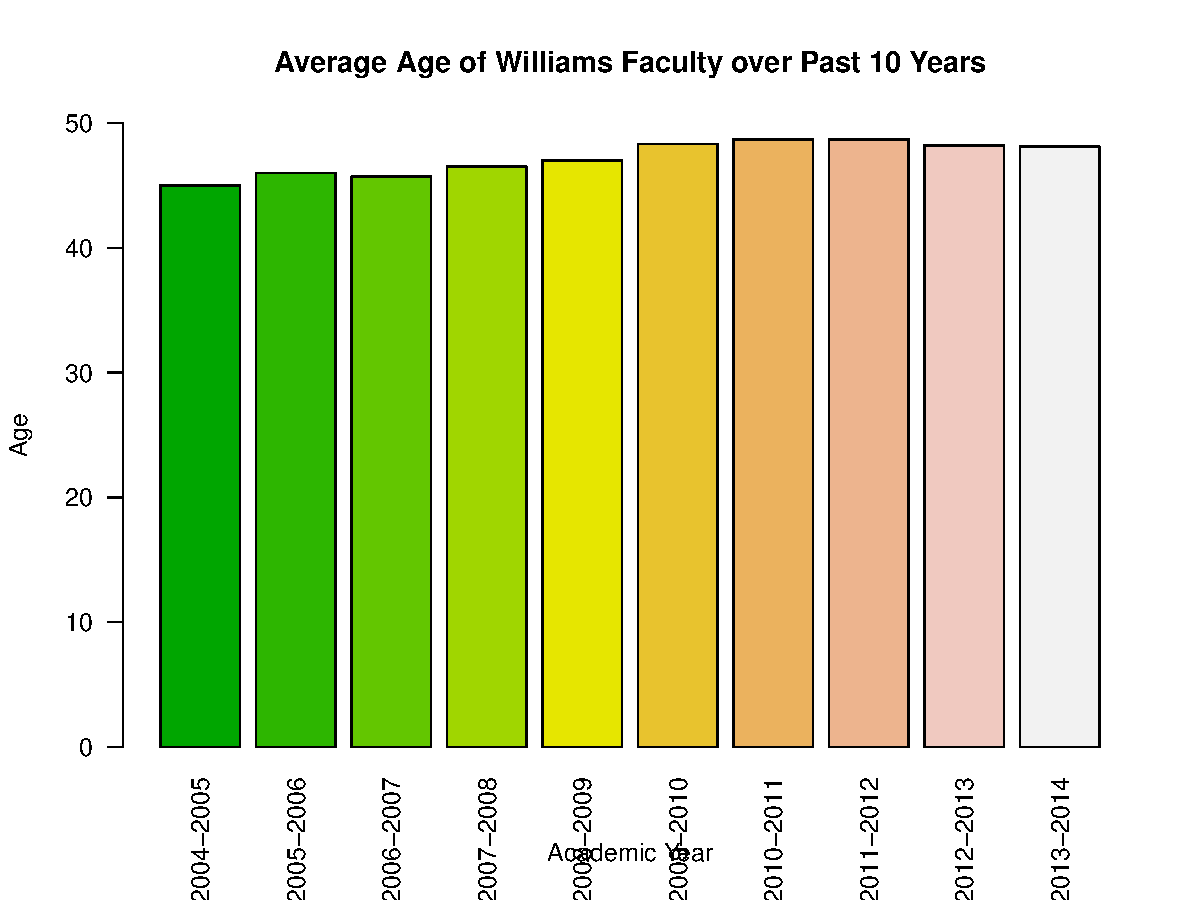
\includegraphics[width=\maxwidth]{figure/unnamed-chunk-6-1} 

\end{knitrout}



\bigskip
The youngest and oldest faculty member's age and name for the last 10 years are as follows:

\bigskip
Youngest 2004-2005 = \(24\), Zafrir Levy, Assistant Professor of Physical Education and Head Coach of Men's and Women's Squash

\bigskip
Oldest 2004-2005 = \(83\), Henry J. Bruton, Visiting Professor of Economics

\bigskip
Youngest 2005-2006 = \(25\), Heather N. Harrington, Assistant Project Cataloger

\bigskip
Oldest 2005-2006 = \(84\), Henry J. Bruton, Visting Professor of Economics

\bigskip
Youngest 2006-2007 = \(25\), Robert Michelin, Visting Lecturer in Music and Director of Zambezi

\bigskip
Oldest 2006-2007 = \(85\), Henry J. Bruton Visting Professor of Economics

\bigskip
Youngest 2007-2008 = \(27\), Heather Harrington, Collections Archivist and Marshall K. Creighton, Lecturer in Physical Education

\bigskip
Oldest 2007-2008 = \(86\), Henry J. Bruton, Visting Professor of Economics

\bigskip
Youngest 2008-2009 = \(23\), Binyavanga Wainaina, Sterling Brown '22 Visiting Professor of Africana Studies, First Semester

\bigskip
Oldest 2008-2009 = \(87\), Henry J. Bruton, Visting Professor of Economics

\bigskip
Youngest 2009-2010 = \(26\), David A. Chalifoux, Library Shelving Facility Supervisor

\bigskip
Oldest 2009-2010 = \(88\), Henry J. Bruton, Visting Professor of Economics

\bigskip
Youngest 2010-2011 = \(24\), Daniel Greenberg, Lecturer of Physical Education and Head Men's Tennis Coach

\bigskip
Oldest 2010-2011 = \(89\), Henry J. Bruton, Visting Professor of Economics

\bigskip
Youngest 2011-2012 = \(25\), Daniel Greenberg, Assistant Professor of Physical Education and Head Men's Tennis Coach

\bigskip
Oldest 2011-2012 = \(90\), Henry J. Bruton, Visting Professor of Economics

\bigskip
Youngest 2012-2013 = \(24\), Qing(Wendy) Wang, Assistant Professor of Statistics

\bigskip
Oldest 2012-2013 = \(91\), Henry J. Bruton, Visting Professor of Economics

\bigskip
Youngest 2013-2014 = \(24\), Sarah A. Mirseyedi, Visiting Lecturer in Art

\bigskip
Oldest 2013-2014 = \(77\), Charles B. Dew, Ephraim Williams Professor of American History

\bigskip
How the Number of Faculty have changed over time? Talk about disclaimer about library



\begin{knitrout}
\definecolor{shadecolor}{rgb}{0.969, 0.969, 0.969}\color{fgcolor}
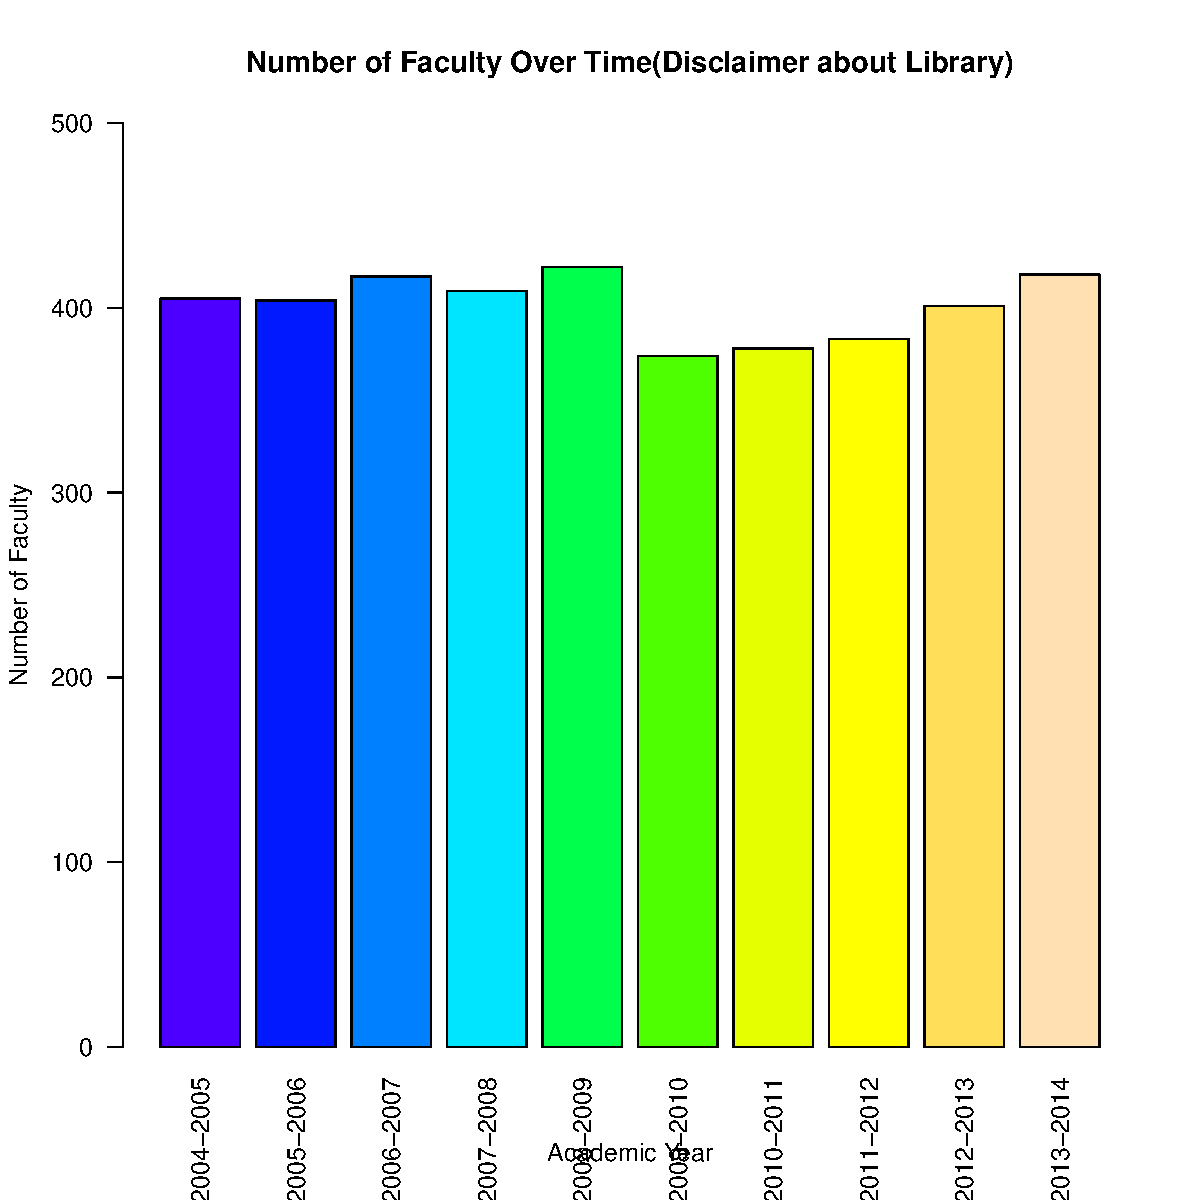
\includegraphics[width=\maxwidth]{figure/unnamed-chunk-8-1} 

\end{knitrout}

\bigskip
How has the age distribution of the professors changed over time?

\begin{knitrout}
\definecolor{shadecolor}{rgb}{0.969, 0.969, 0.969}\color{fgcolor}
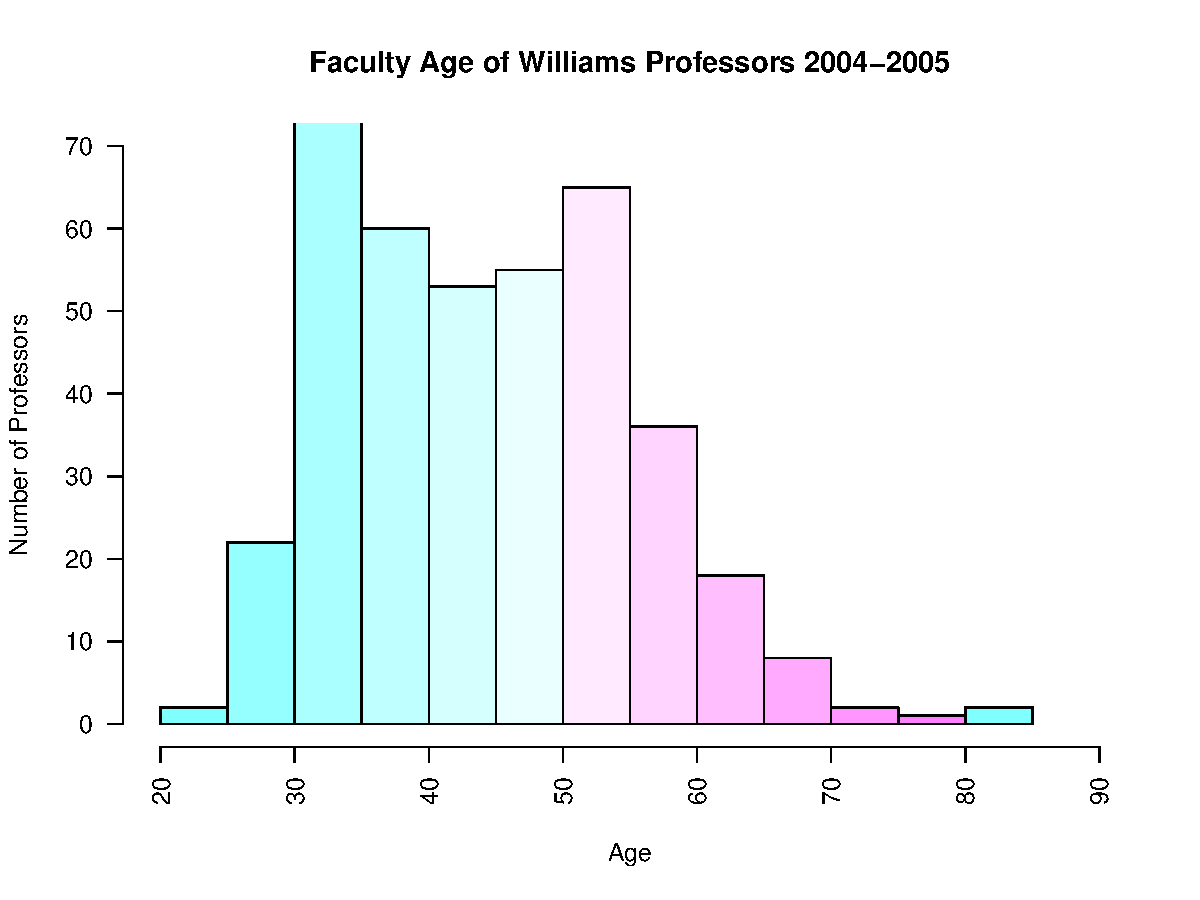
\includegraphics[width=\maxwidth]{figure/unnamed-chunk-9-1} 

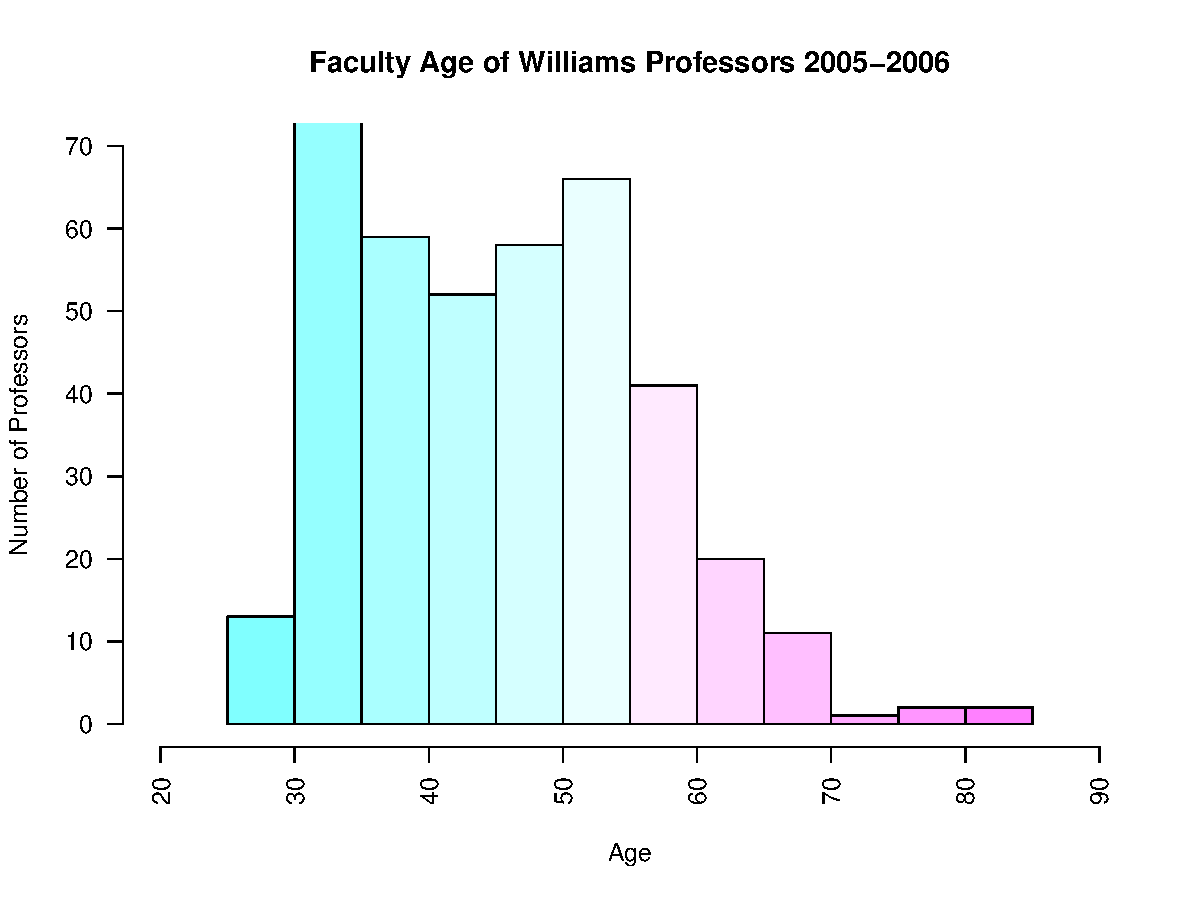
\includegraphics[width=\maxwidth]{figure/unnamed-chunk-9-2} 

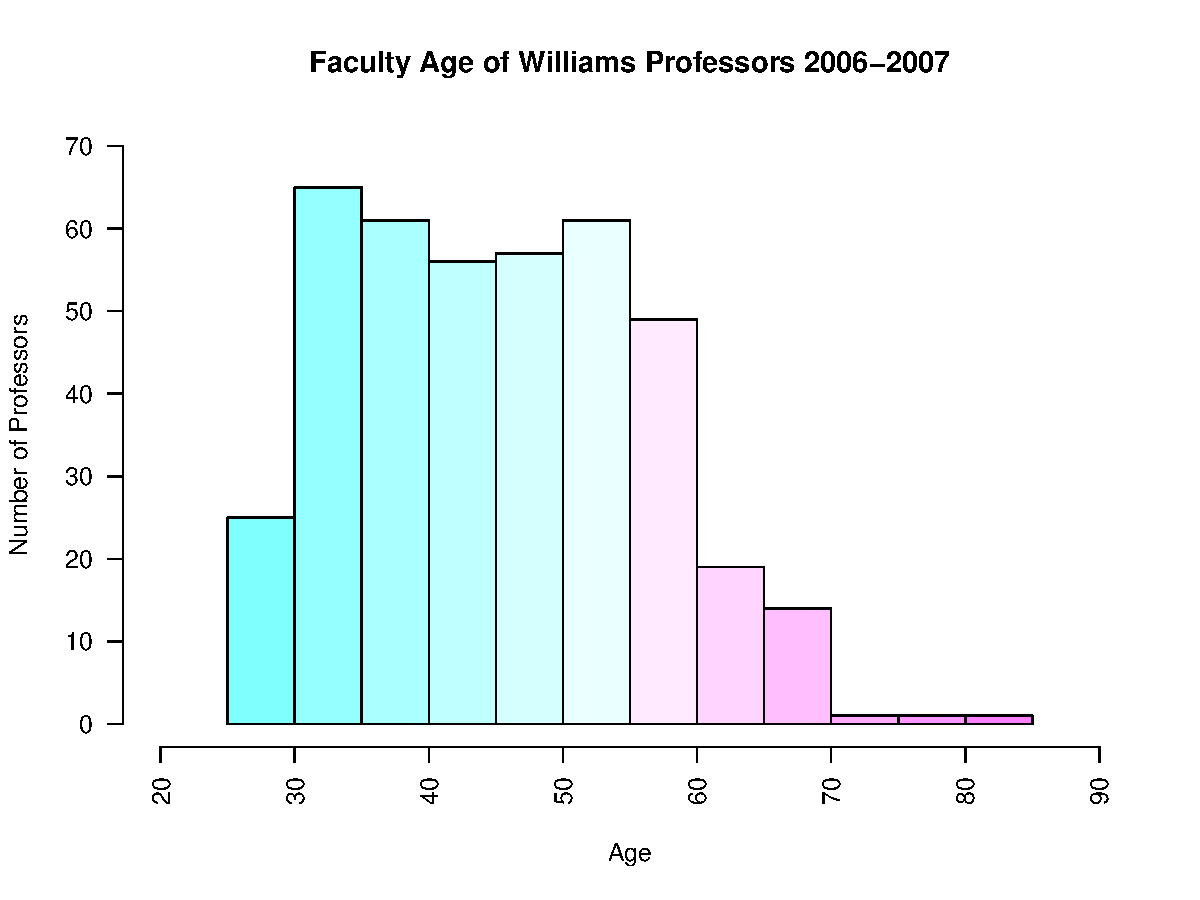
\includegraphics[width=\maxwidth]{figure/unnamed-chunk-9-3} 

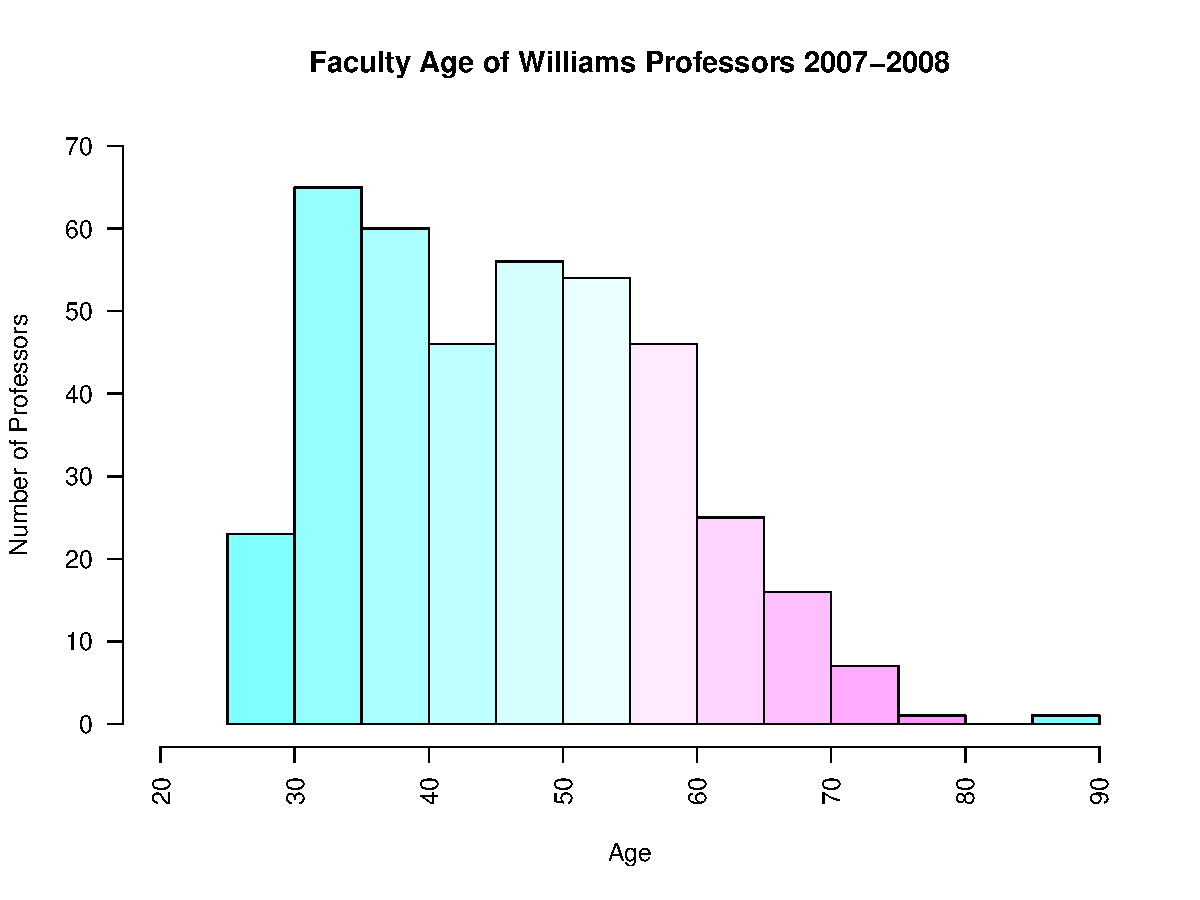
\includegraphics[width=\maxwidth]{figure/unnamed-chunk-9-4} 

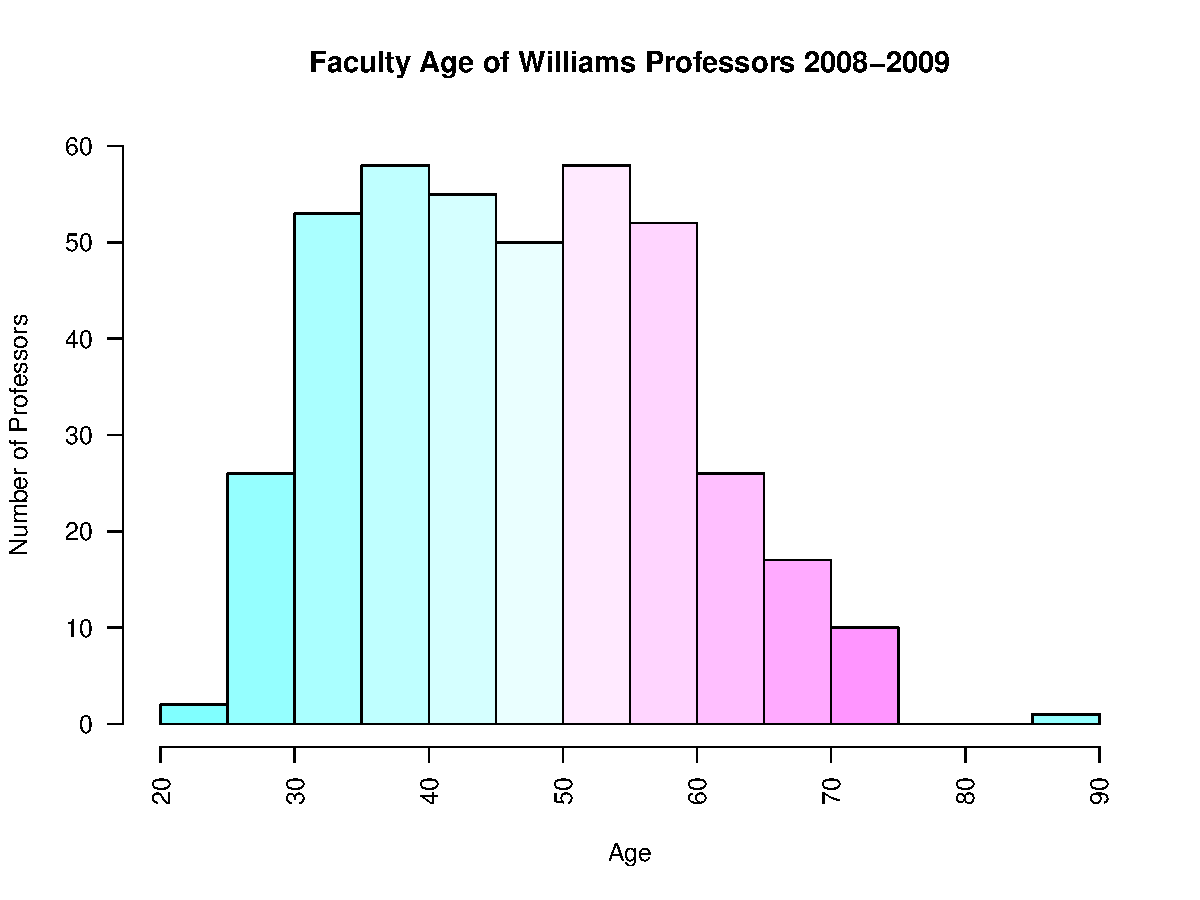
\includegraphics[width=\maxwidth]{figure/unnamed-chunk-9-5} 

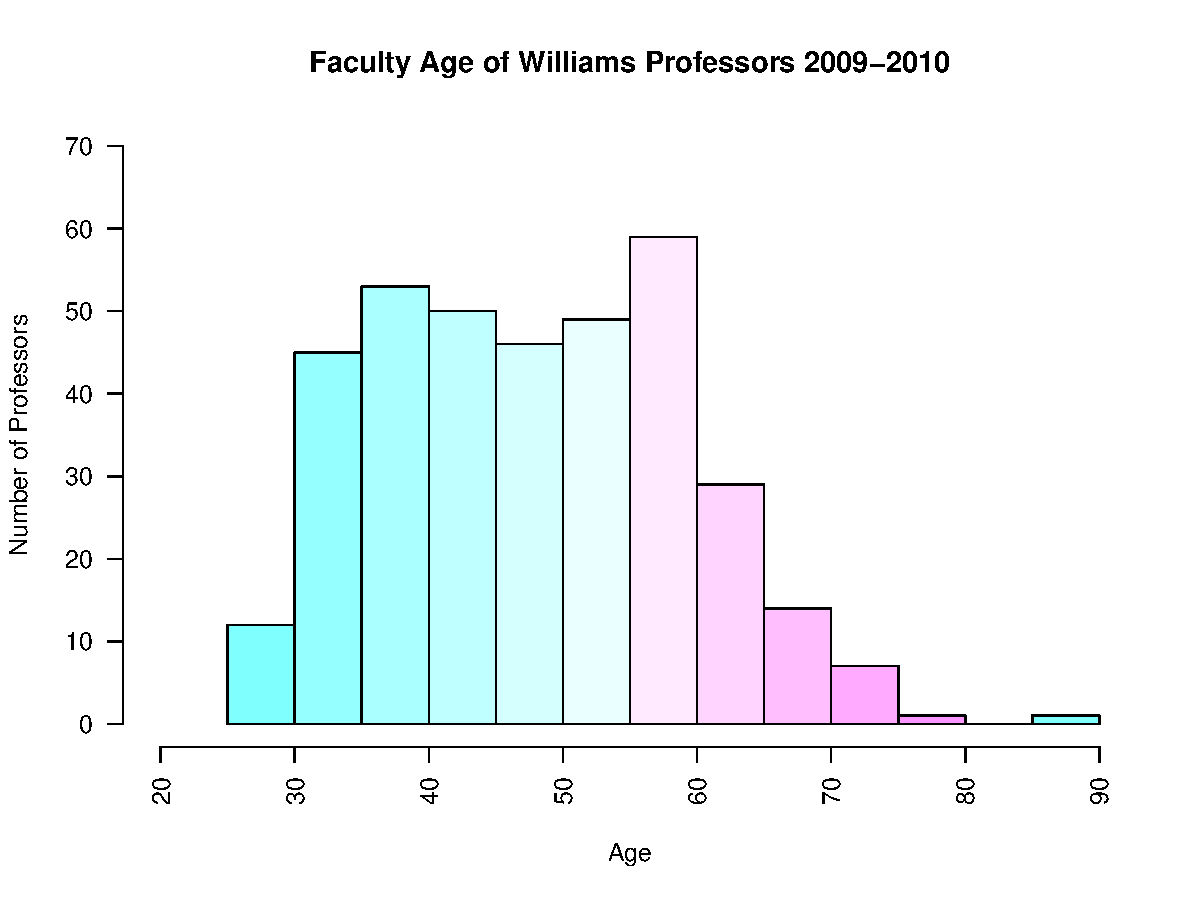
\includegraphics[width=\maxwidth]{figure/unnamed-chunk-9-6} 

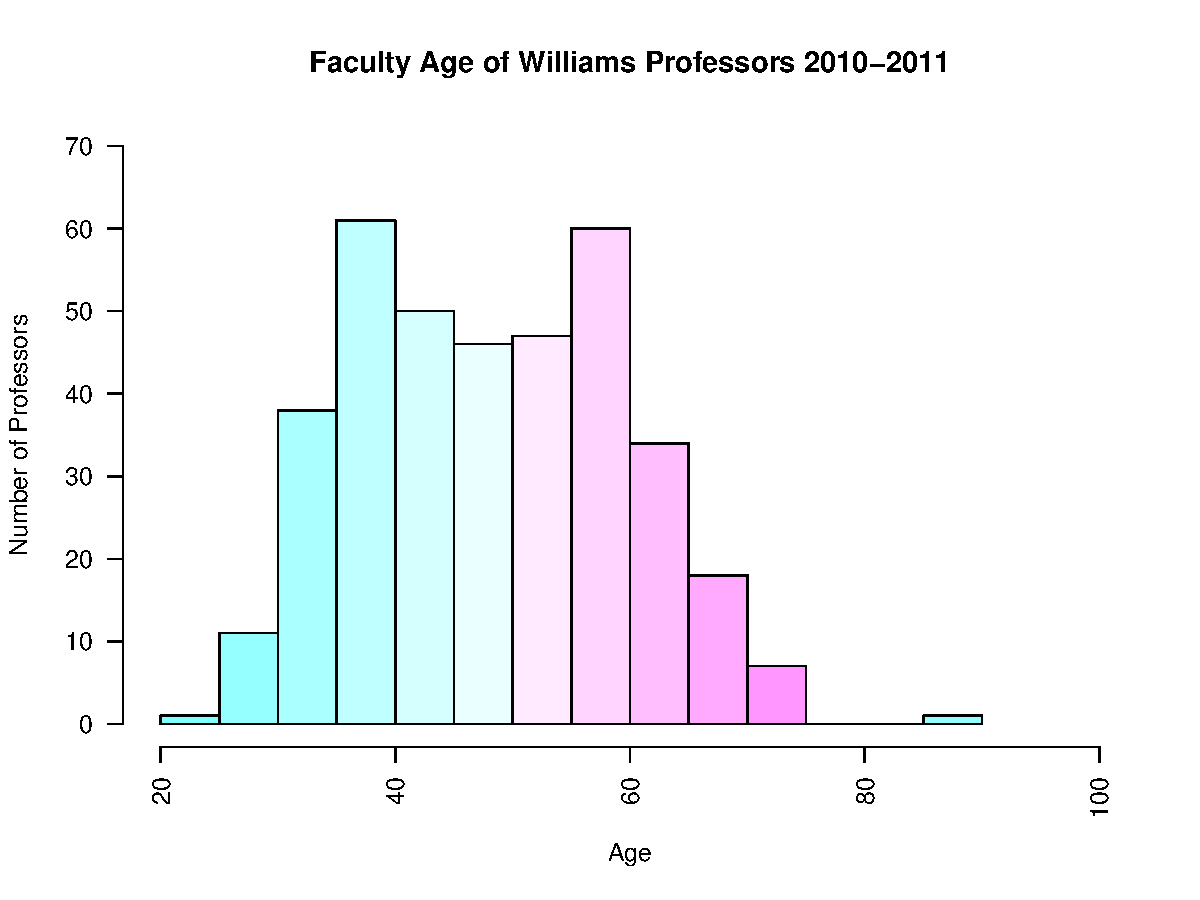
\includegraphics[width=\maxwidth]{figure/unnamed-chunk-9-7} 

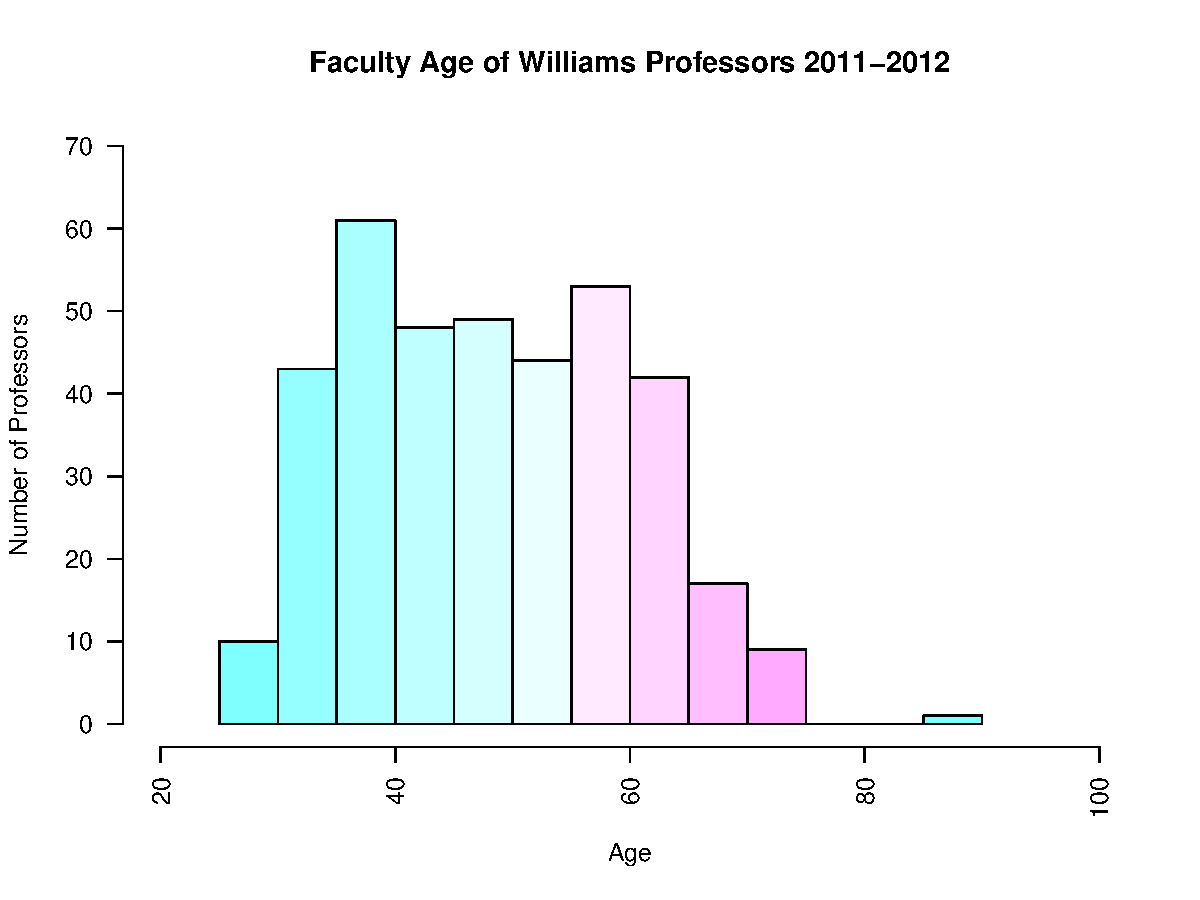
\includegraphics[width=\maxwidth]{figure/unnamed-chunk-9-8} 

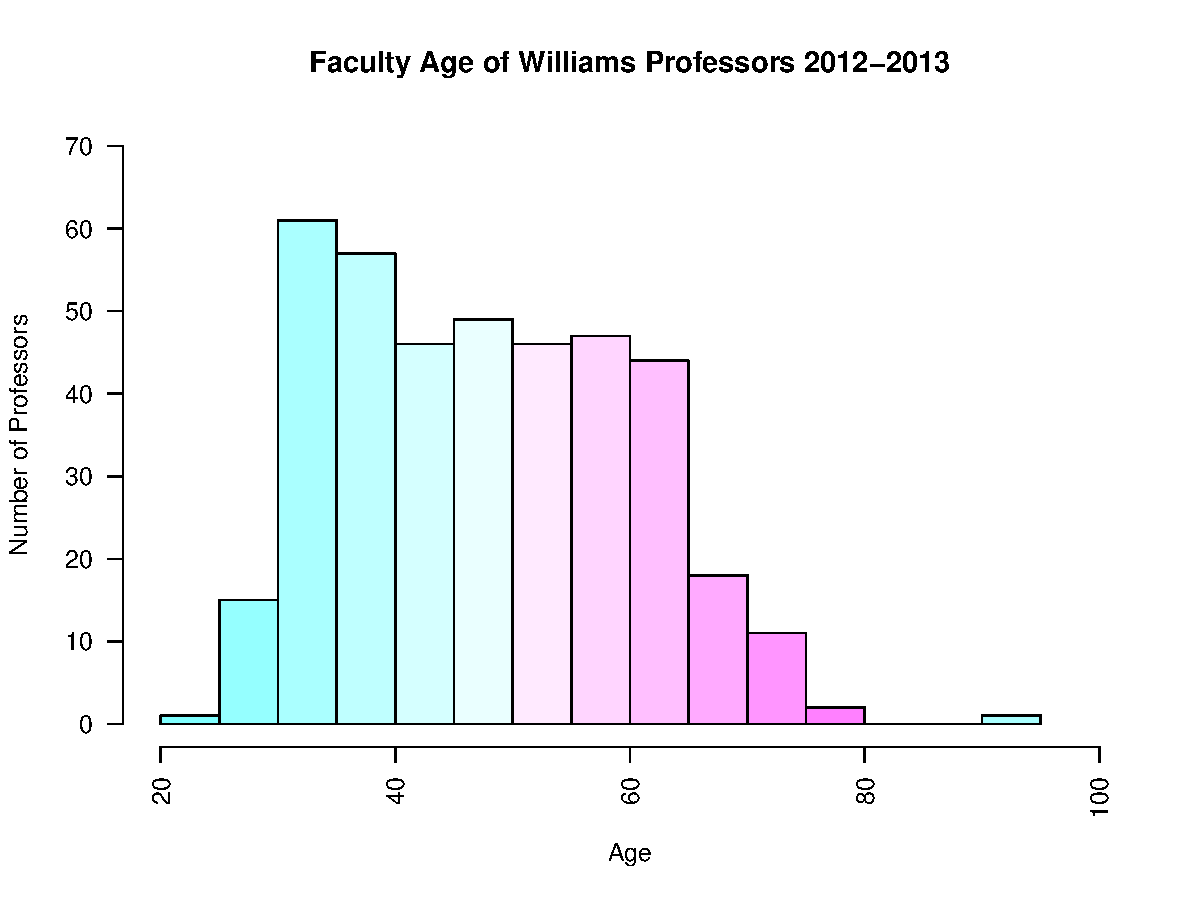
\includegraphics[width=\maxwidth]{figure/unnamed-chunk-9-9} 

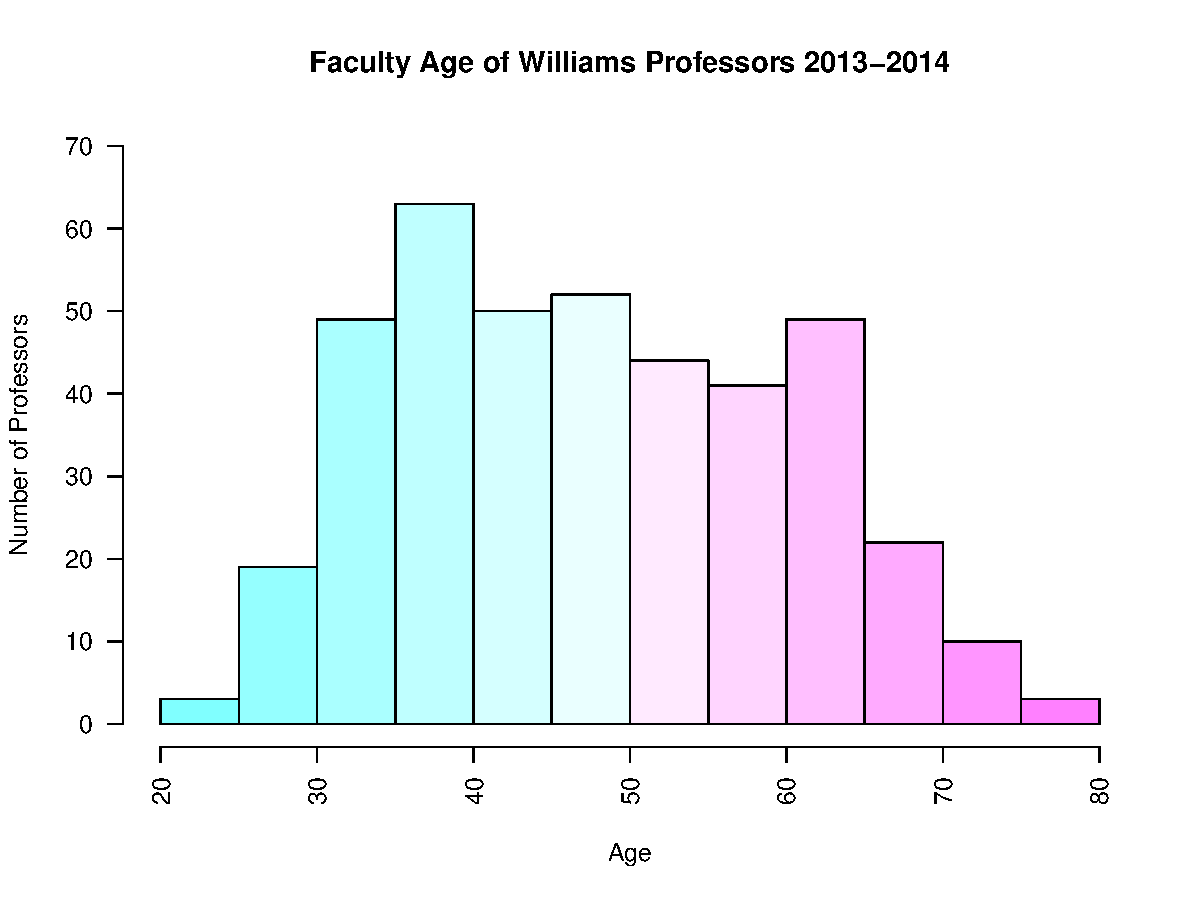
\includegraphics[width=\maxwidth]{figure/unnamed-chunk-9-10} 

\end{knitrout}

\bigskip
Average Ages by Department??

\begin{knitrout}
\definecolor{shadecolor}{rgb}{0.969, 0.969, 0.969}\color{fgcolor}
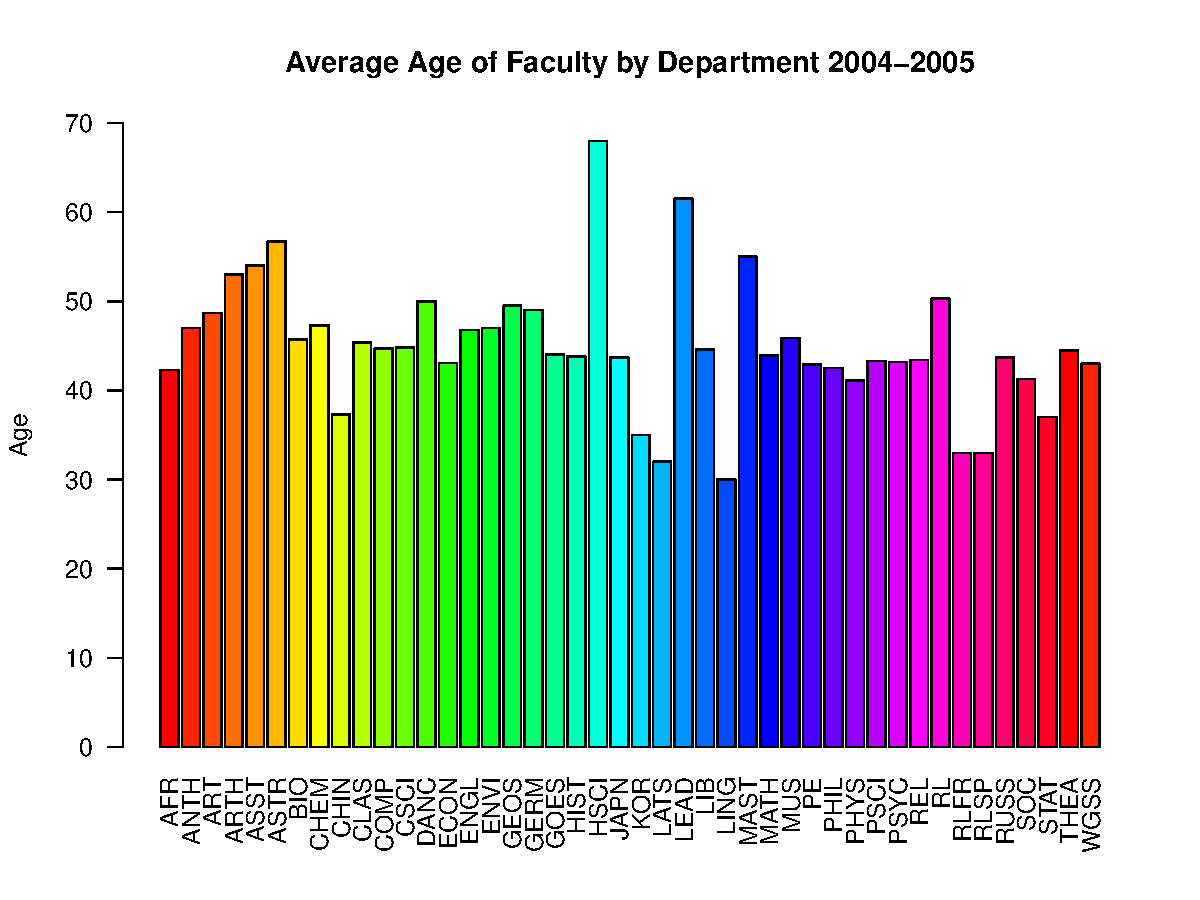
\includegraphics[width=\maxwidth]{figure/unnamed-chunk-10-1} 

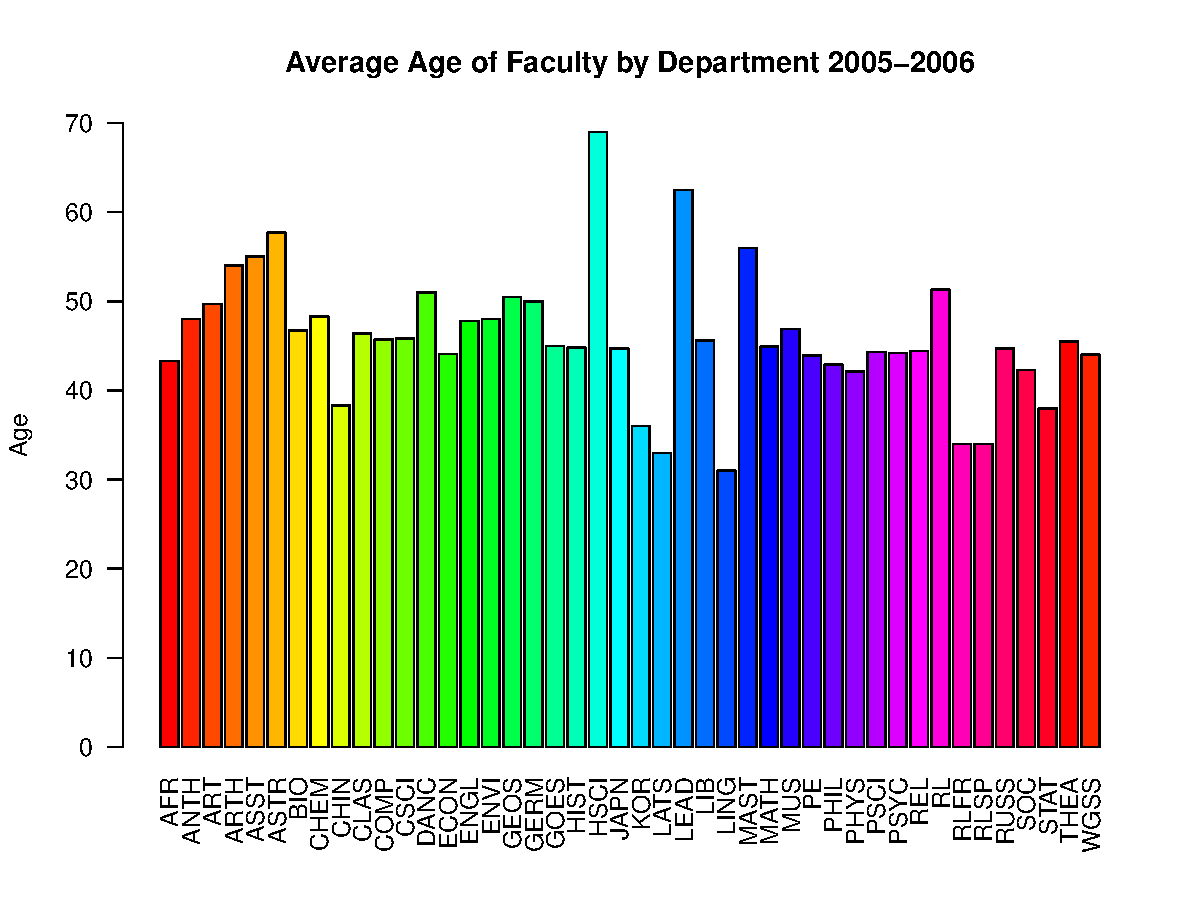
\includegraphics[width=\maxwidth]{figure/unnamed-chunk-10-2} 

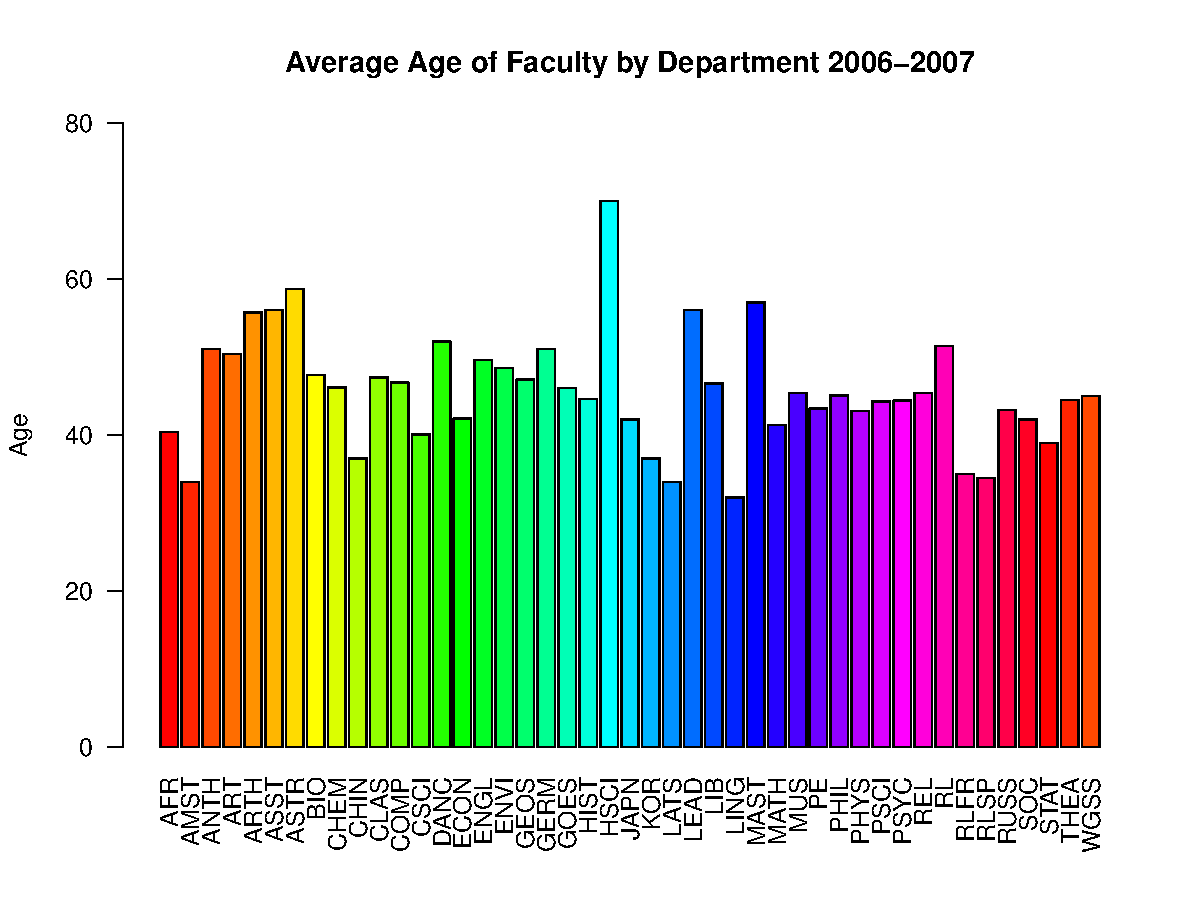
\includegraphics[width=\maxwidth]{figure/unnamed-chunk-10-3} 

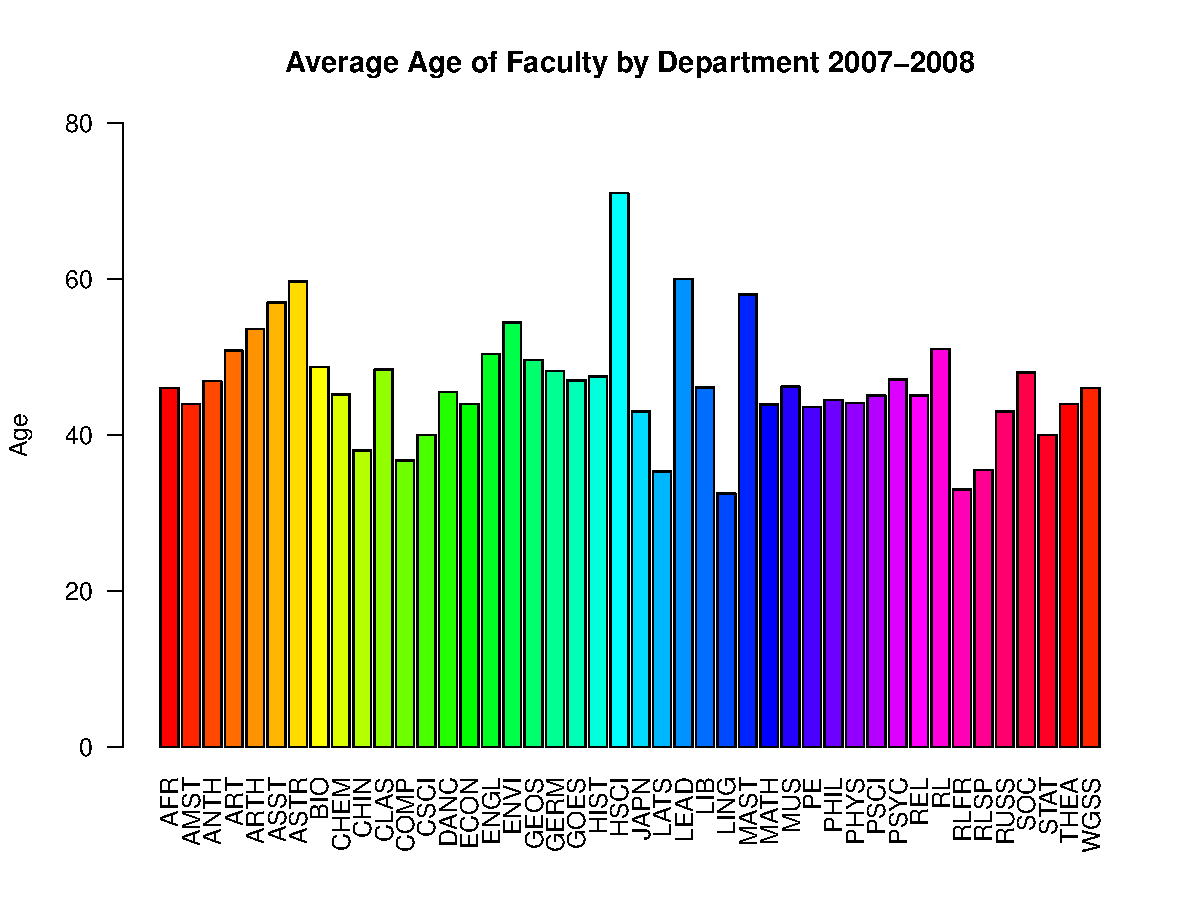
\includegraphics[width=\maxwidth]{figure/unnamed-chunk-10-4} 

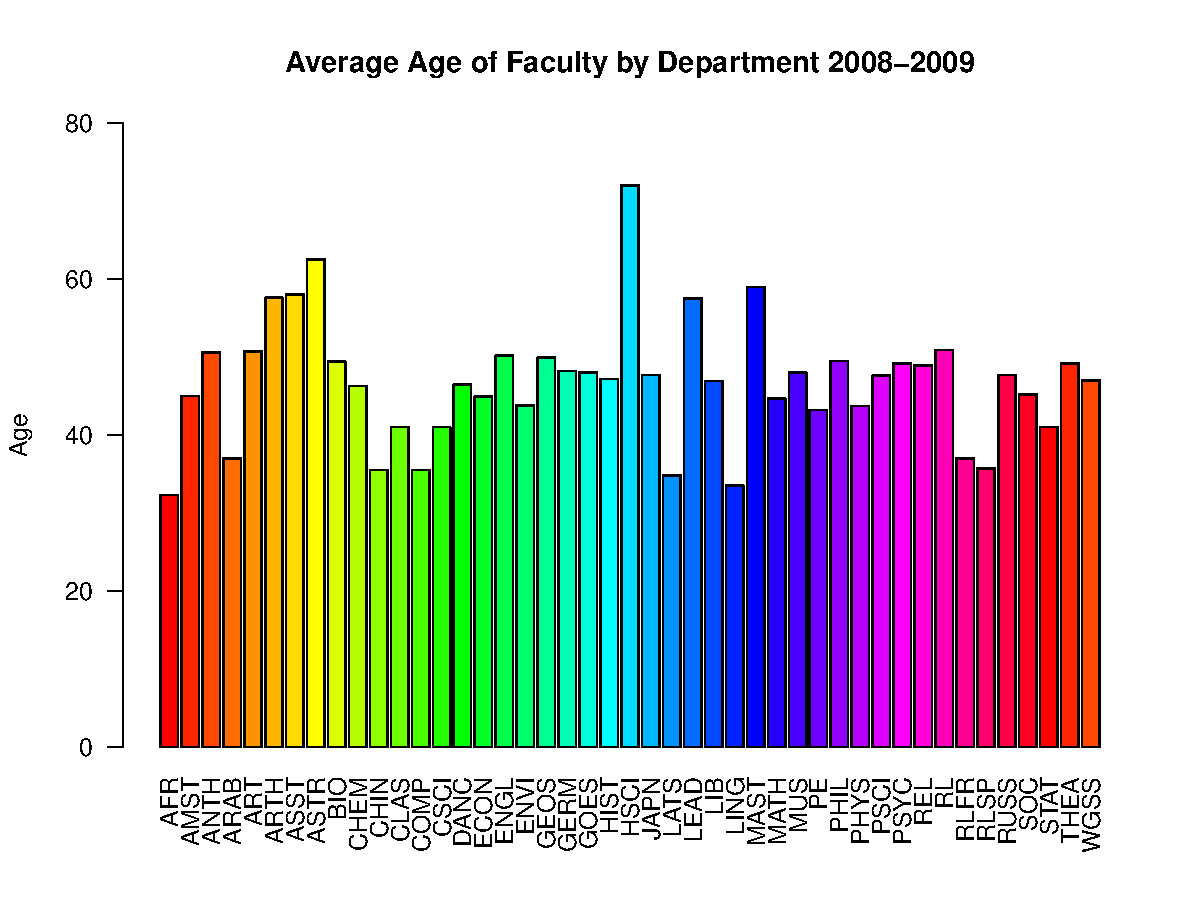
\includegraphics[width=\maxwidth]{figure/unnamed-chunk-10-5} 

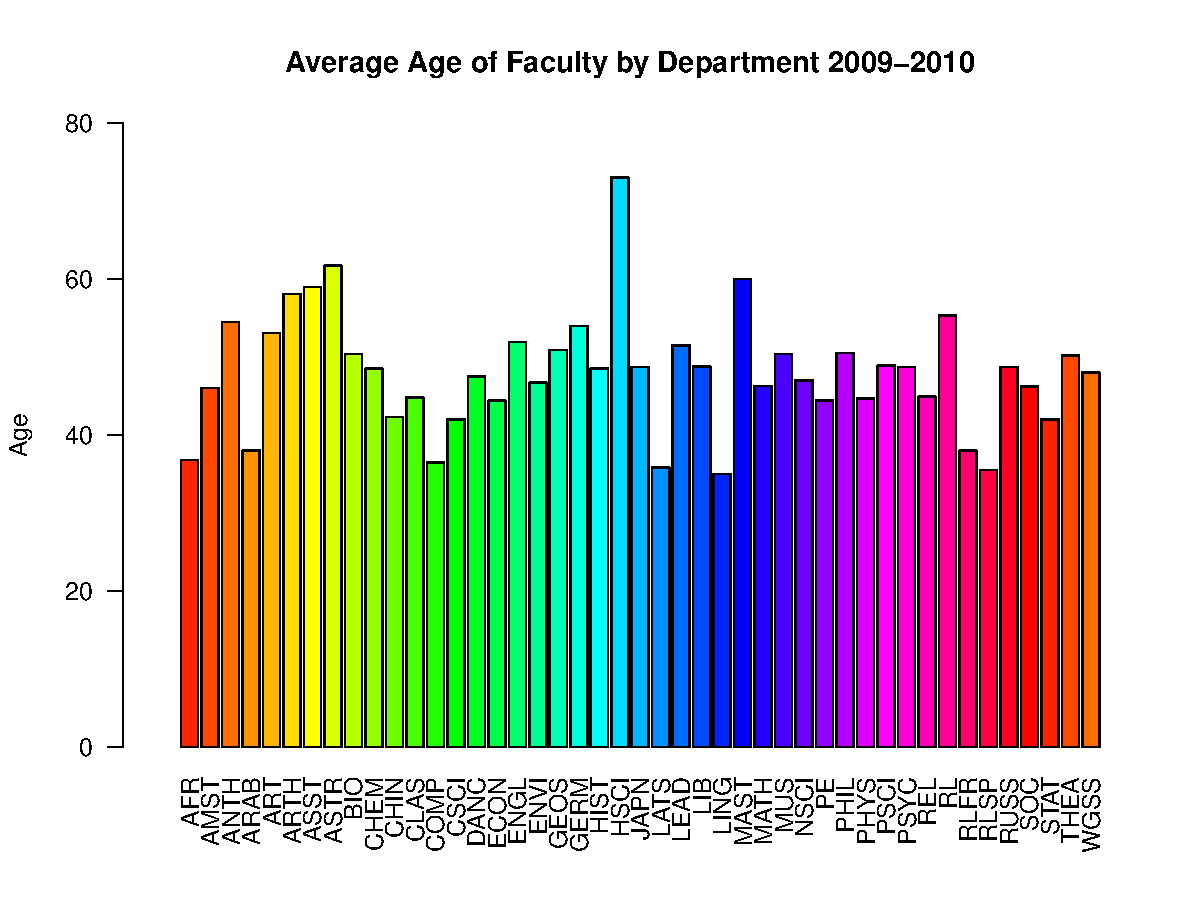
\includegraphics[width=\maxwidth]{figure/unnamed-chunk-10-6} 

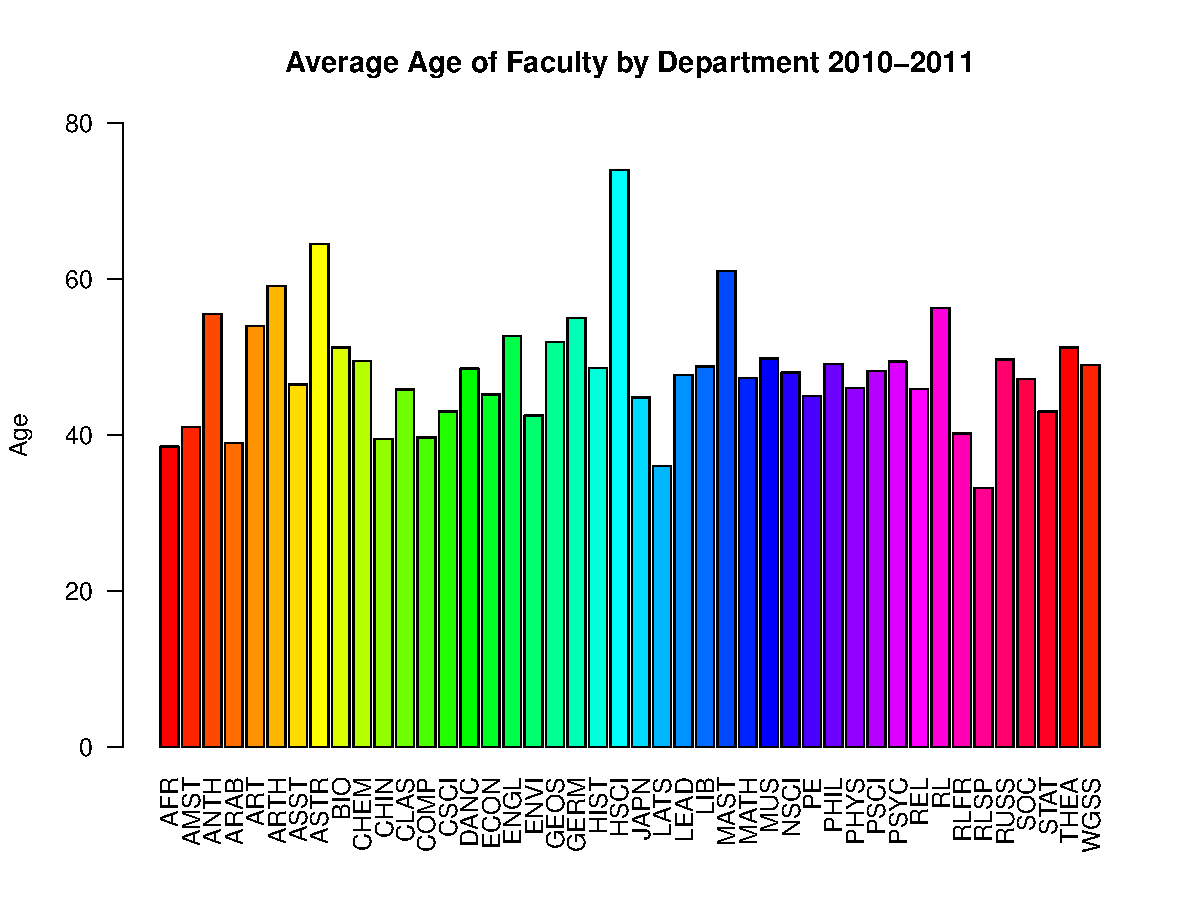
\includegraphics[width=\maxwidth]{figure/unnamed-chunk-10-7} 

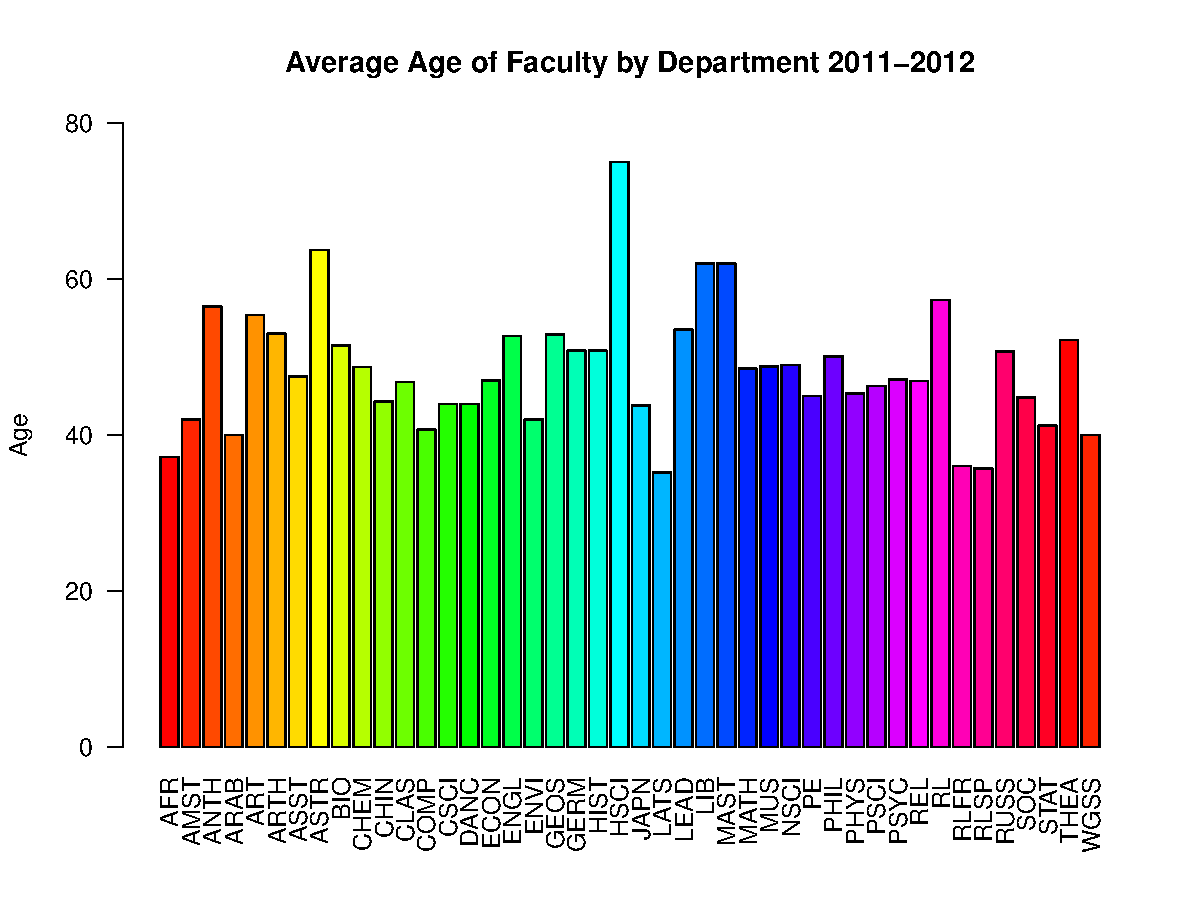
\includegraphics[width=\maxwidth]{figure/unnamed-chunk-10-8} 

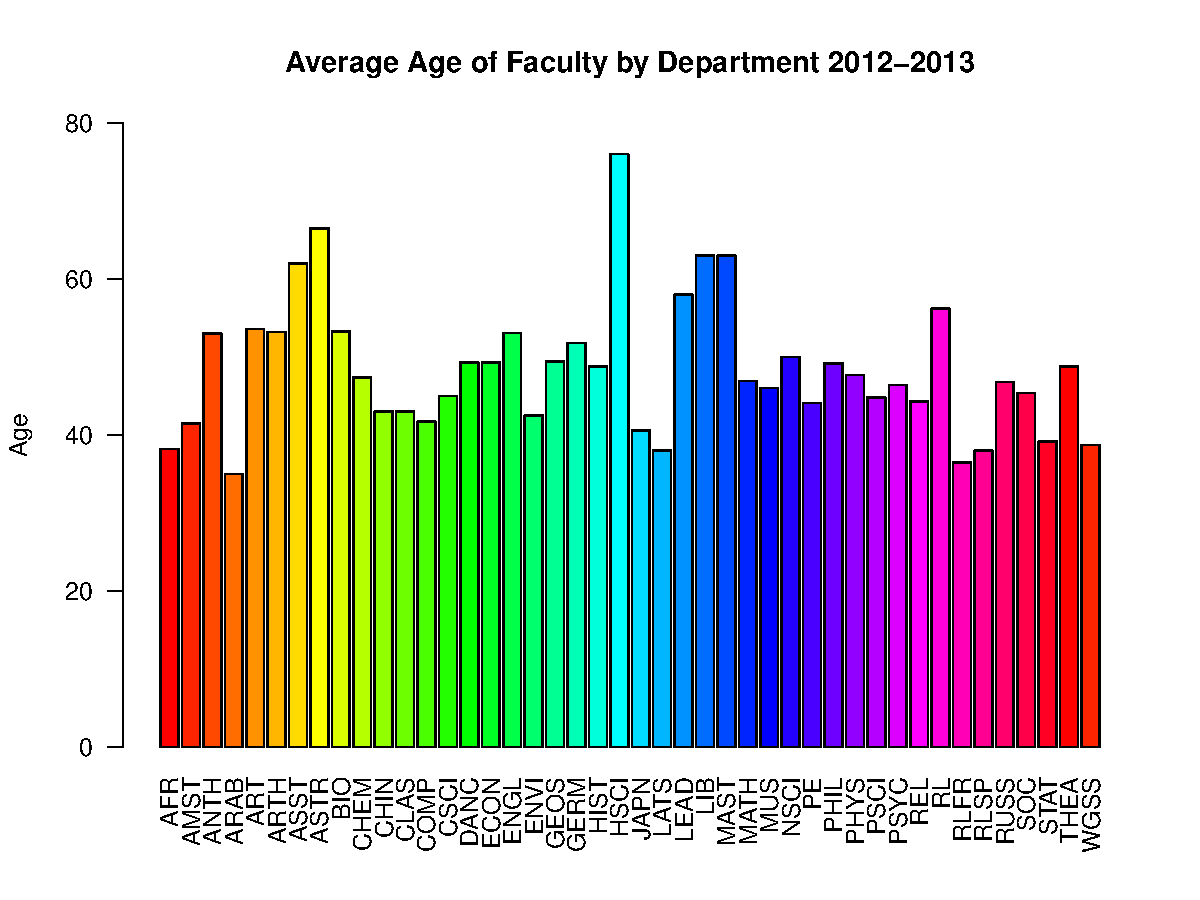
\includegraphics[width=\maxwidth]{figure/unnamed-chunk-10-9} 

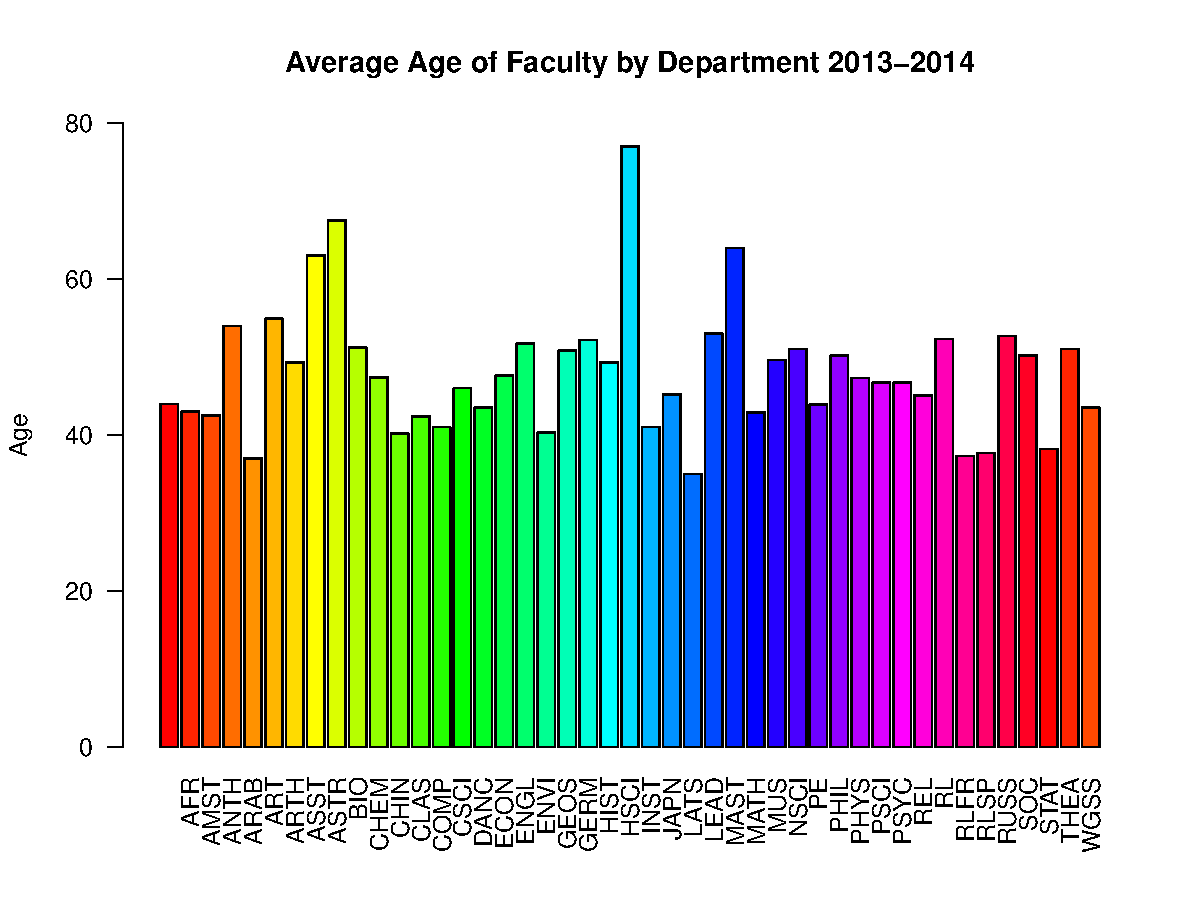
\includegraphics[width=\maxwidth]{figure/unnamed-chunk-10-10} 

\end{knitrout}

\bigskip
How do the ages differ by gender?

\begin{knitrout}
\definecolor{shadecolor}{rgb}{0.969, 0.969, 0.969}\color{fgcolor}
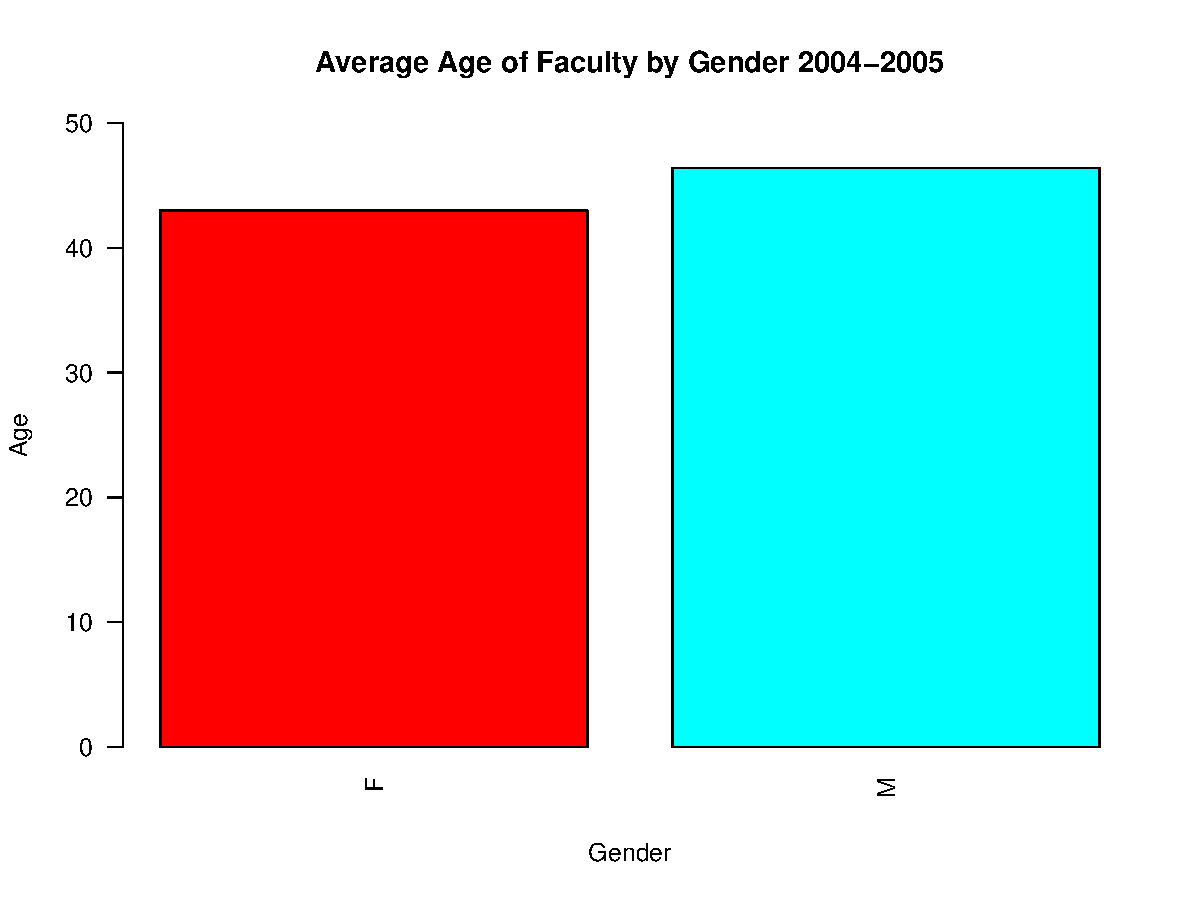
\includegraphics[width=\maxwidth]{figure/unnamed-chunk-11-1} 

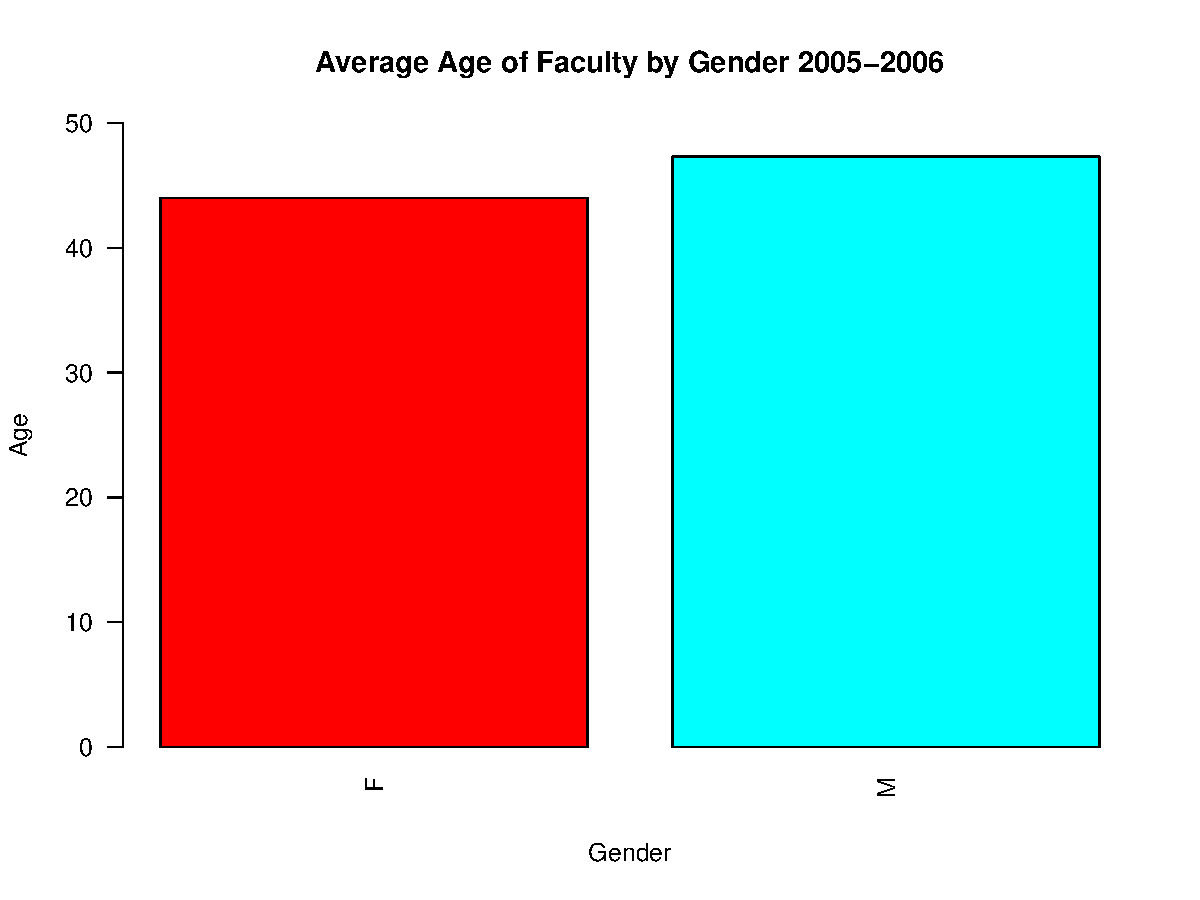
\includegraphics[width=\maxwidth]{figure/unnamed-chunk-11-2} 

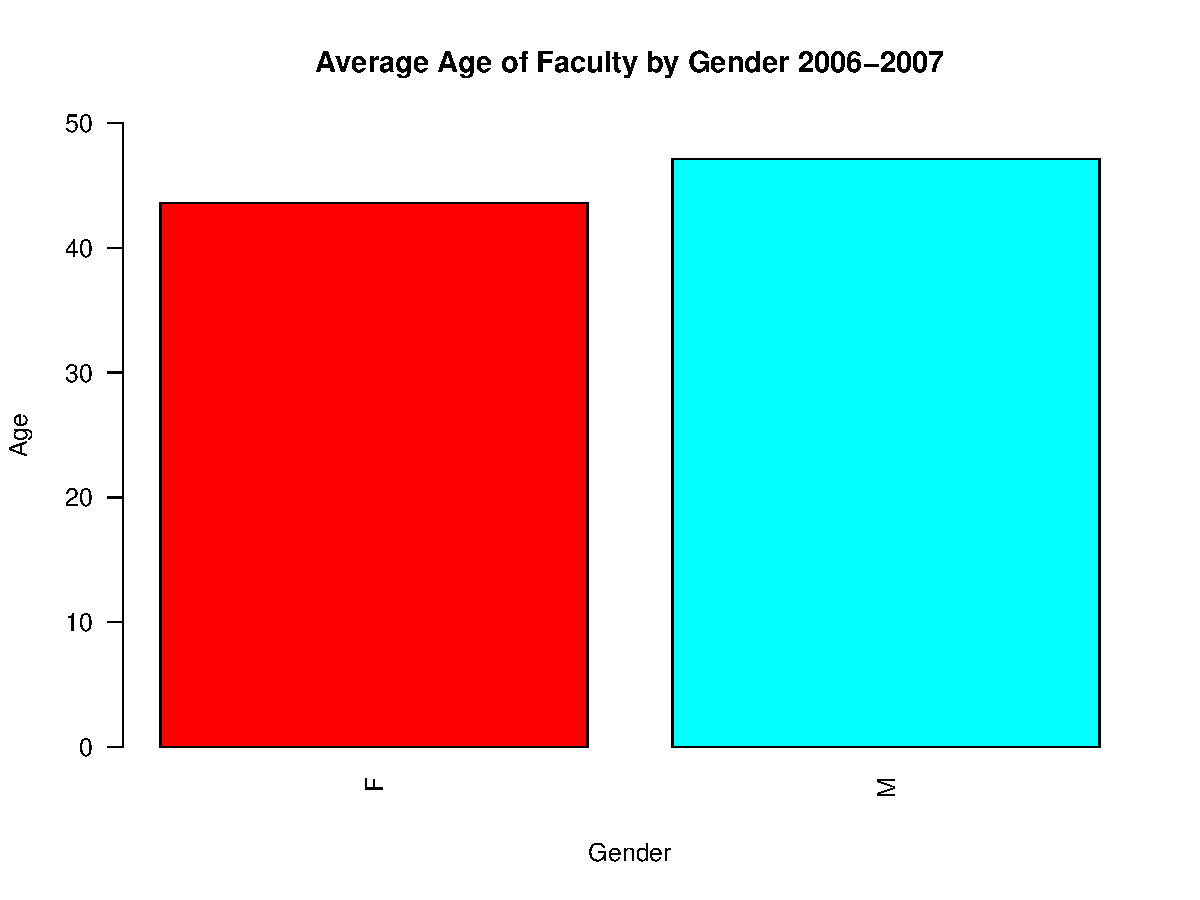
\includegraphics[width=\maxwidth]{figure/unnamed-chunk-11-3} 

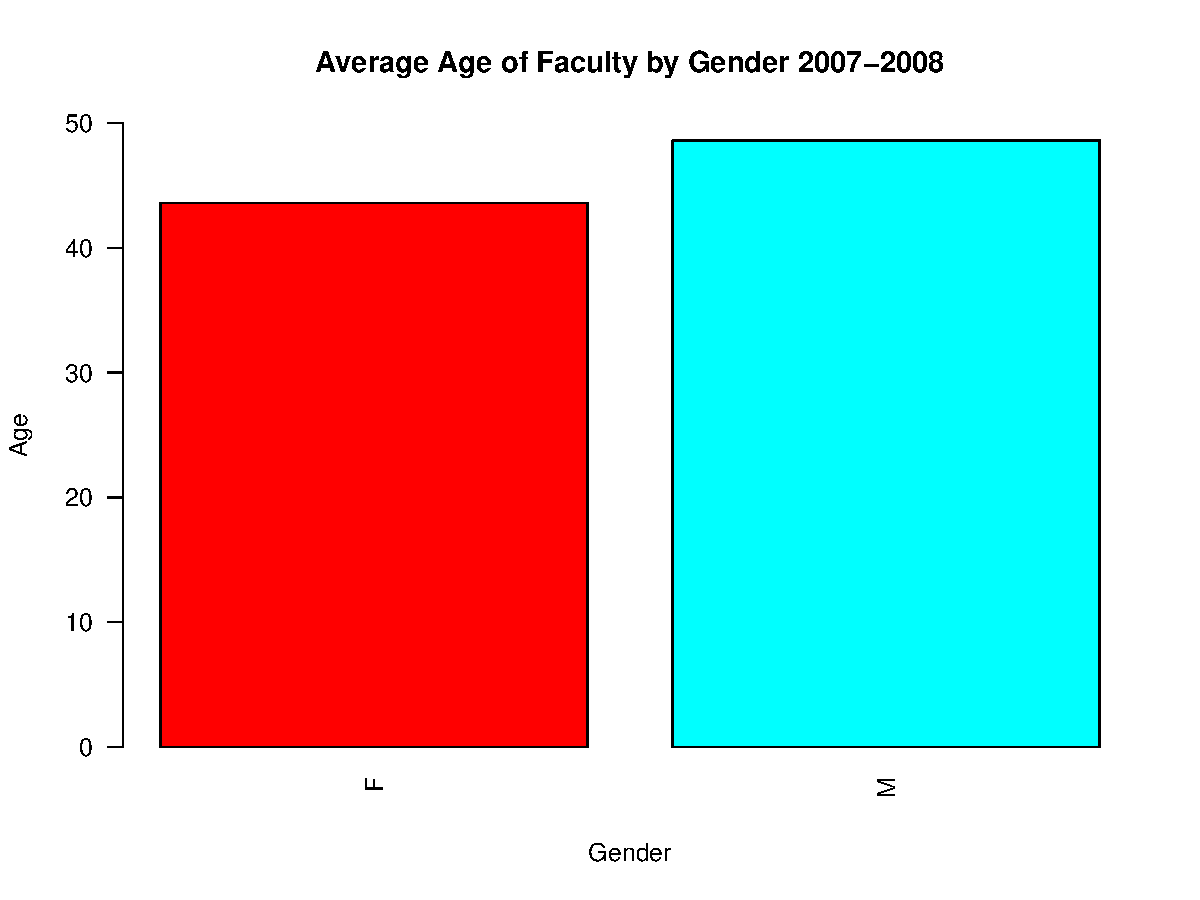
\includegraphics[width=\maxwidth]{figure/unnamed-chunk-11-4} 

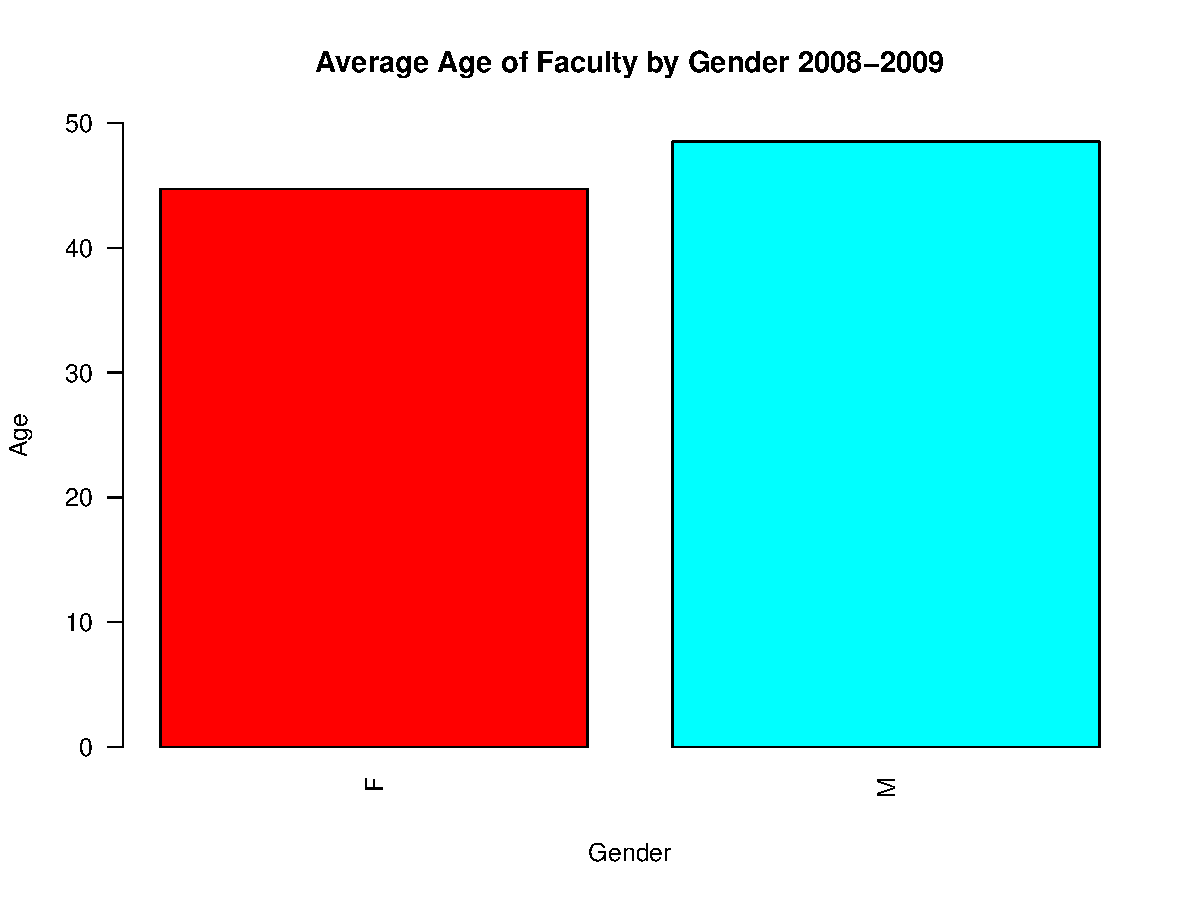
\includegraphics[width=\maxwidth]{figure/unnamed-chunk-11-5} 

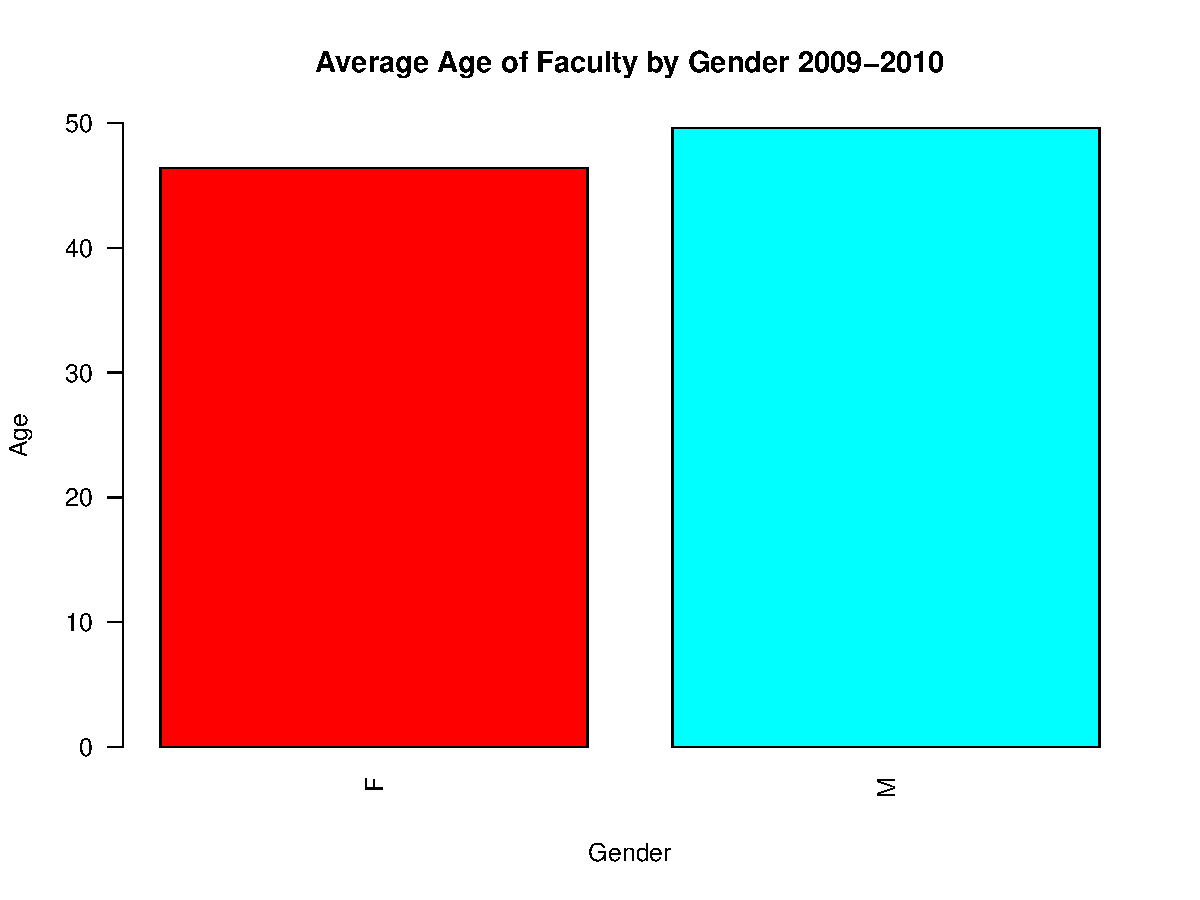
\includegraphics[width=\maxwidth]{figure/unnamed-chunk-11-6} 

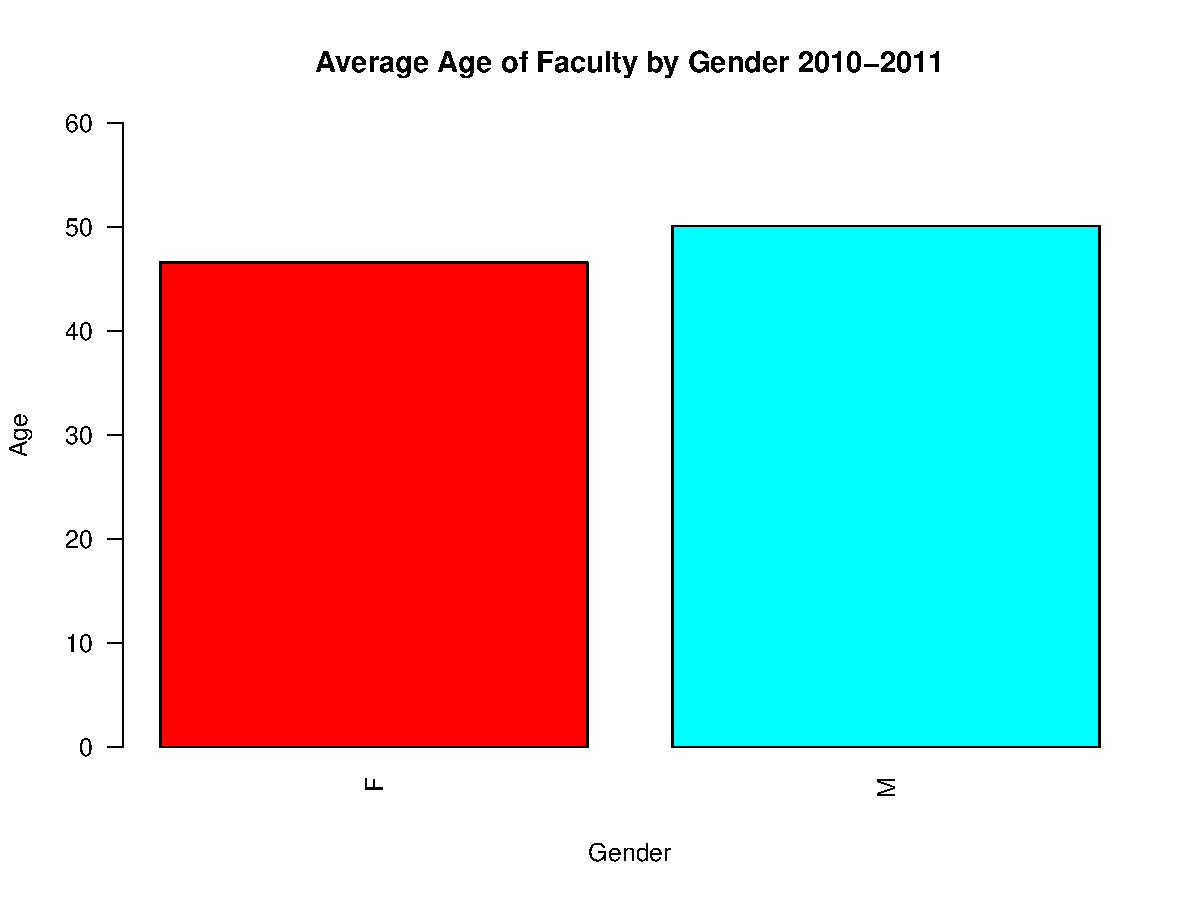
\includegraphics[width=\maxwidth]{figure/unnamed-chunk-11-7} 

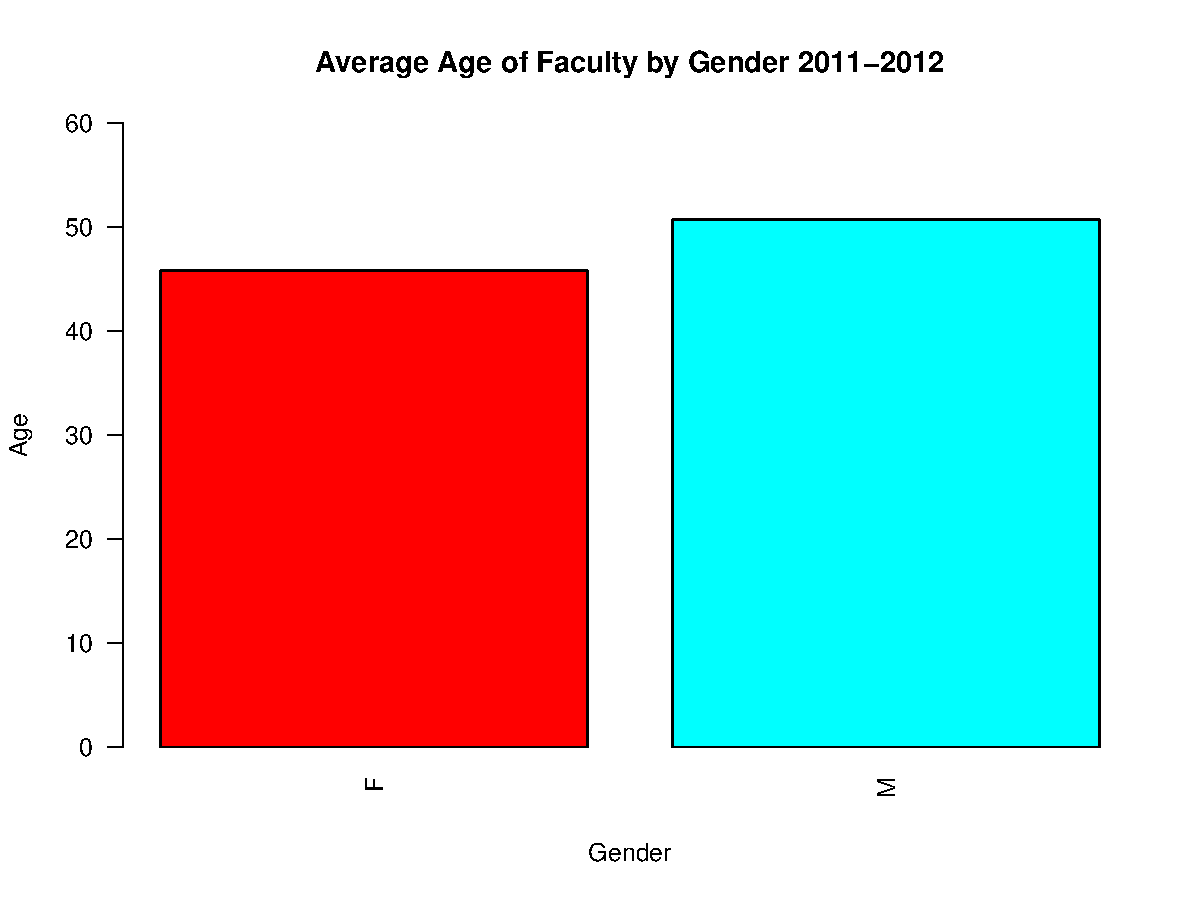
\includegraphics[width=\maxwidth]{figure/unnamed-chunk-11-8} 

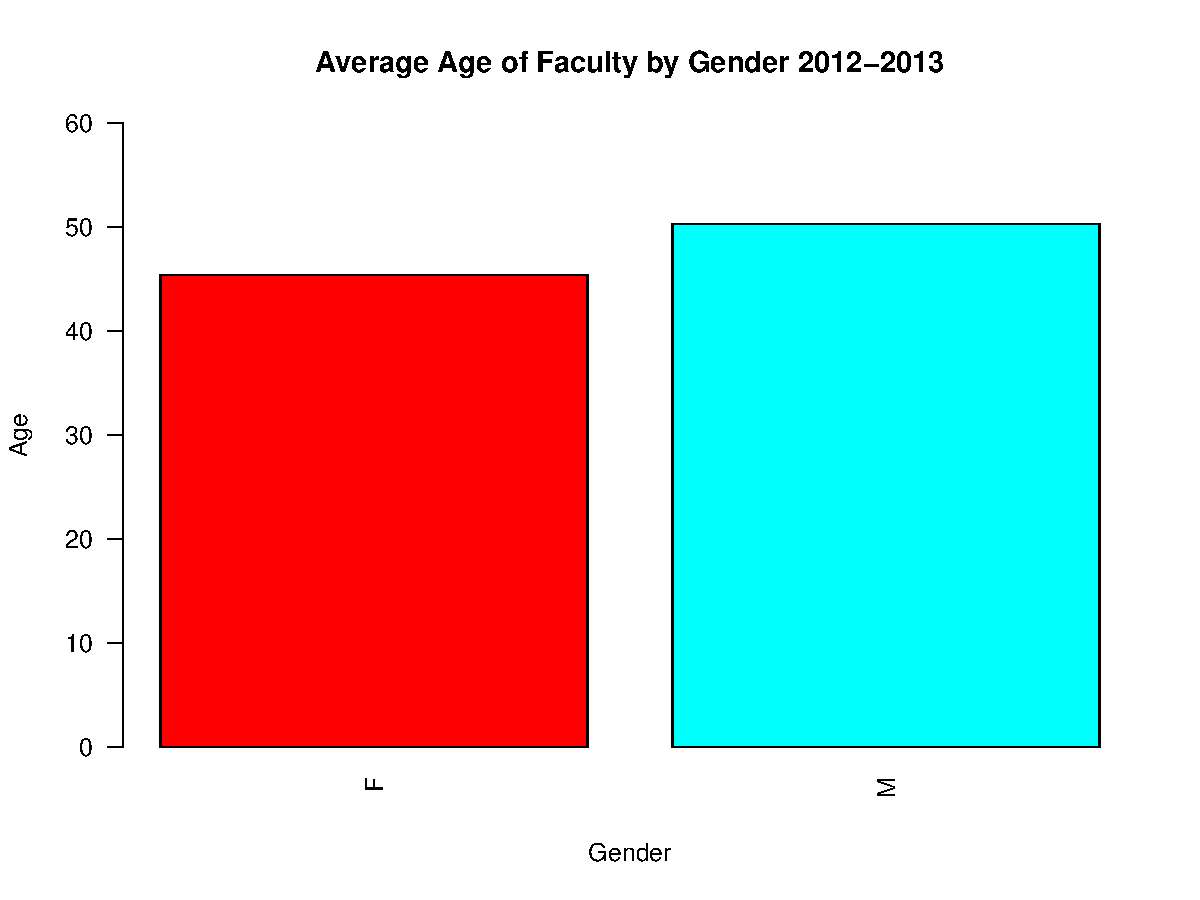
\includegraphics[width=\maxwidth]{figure/unnamed-chunk-11-9} 

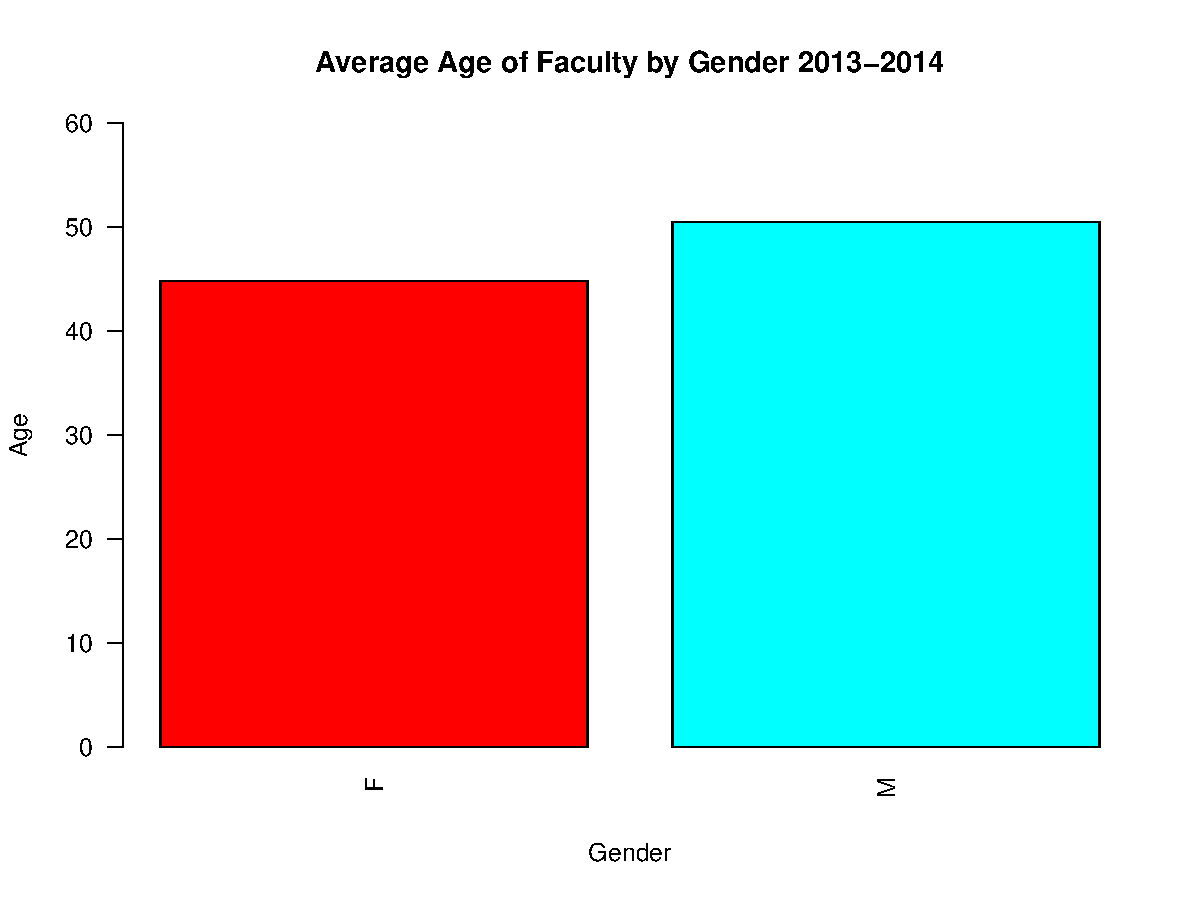
\includegraphics[width=\maxwidth]{figure/unnamed-chunk-11-10} 

\end{knitrout}

\bigskip
How High is the Correlation between Age and Year of Terminal Degree.

\begin{knitrout}
\definecolor{shadecolor}{rgb}{0.969, 0.969, 0.969}\color{fgcolor}
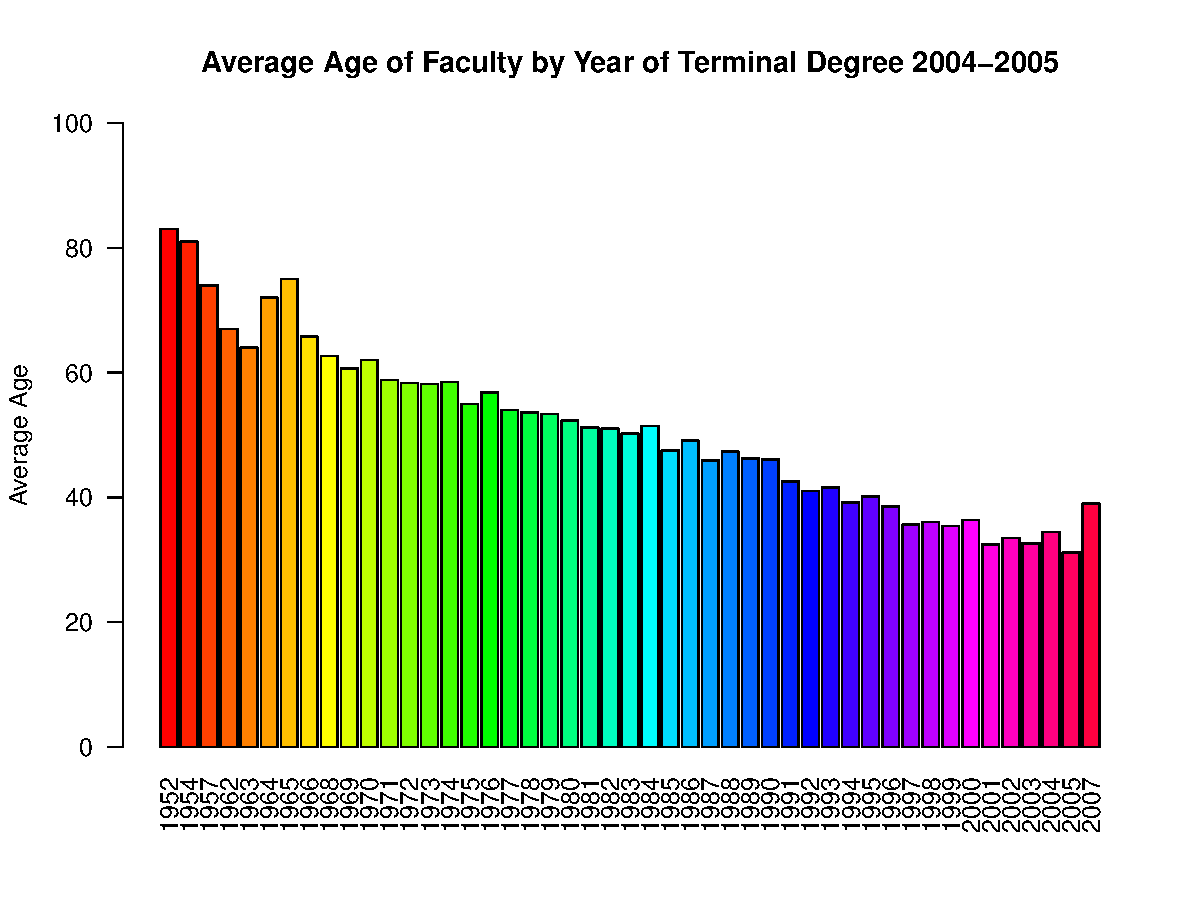
\includegraphics[width=\maxwidth]{figure/unnamed-chunk-12-1} 

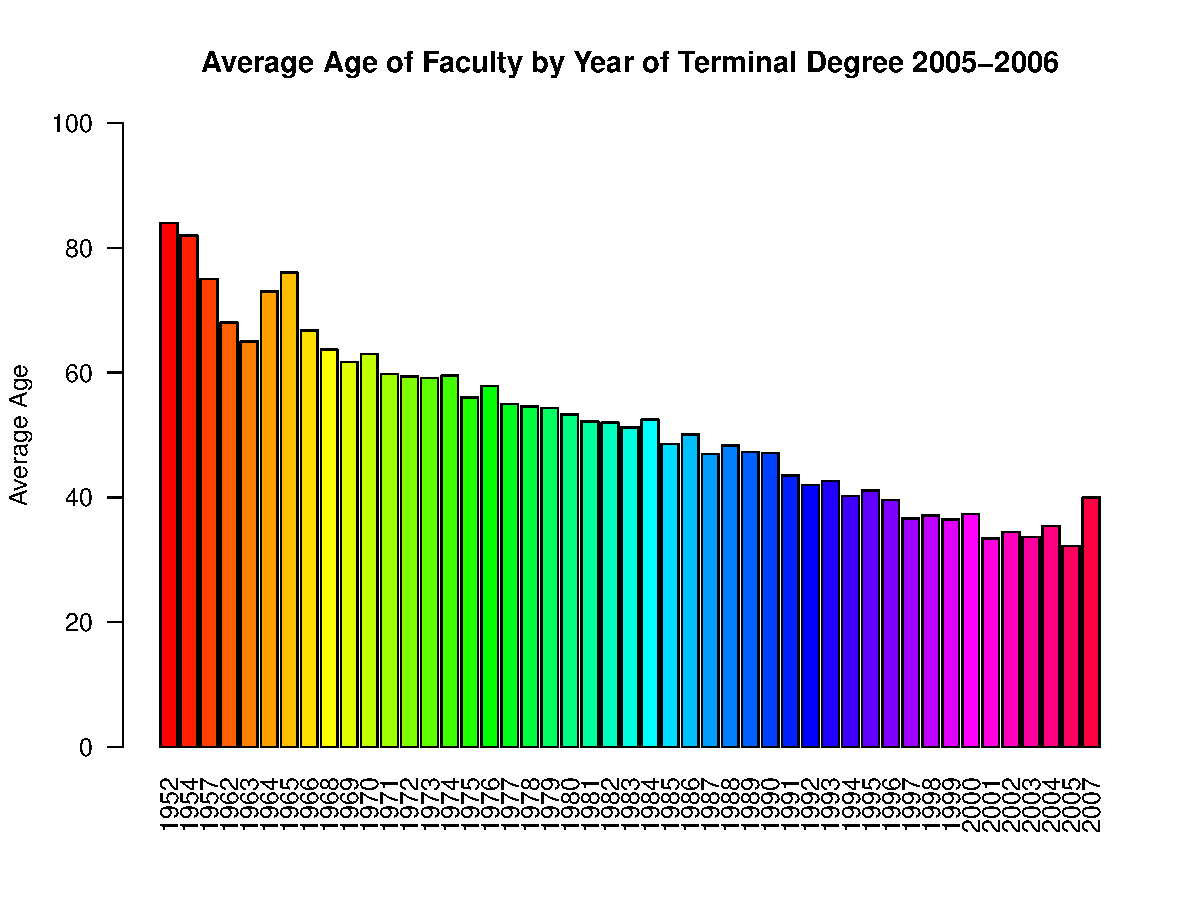
\includegraphics[width=\maxwidth]{figure/unnamed-chunk-12-2} 

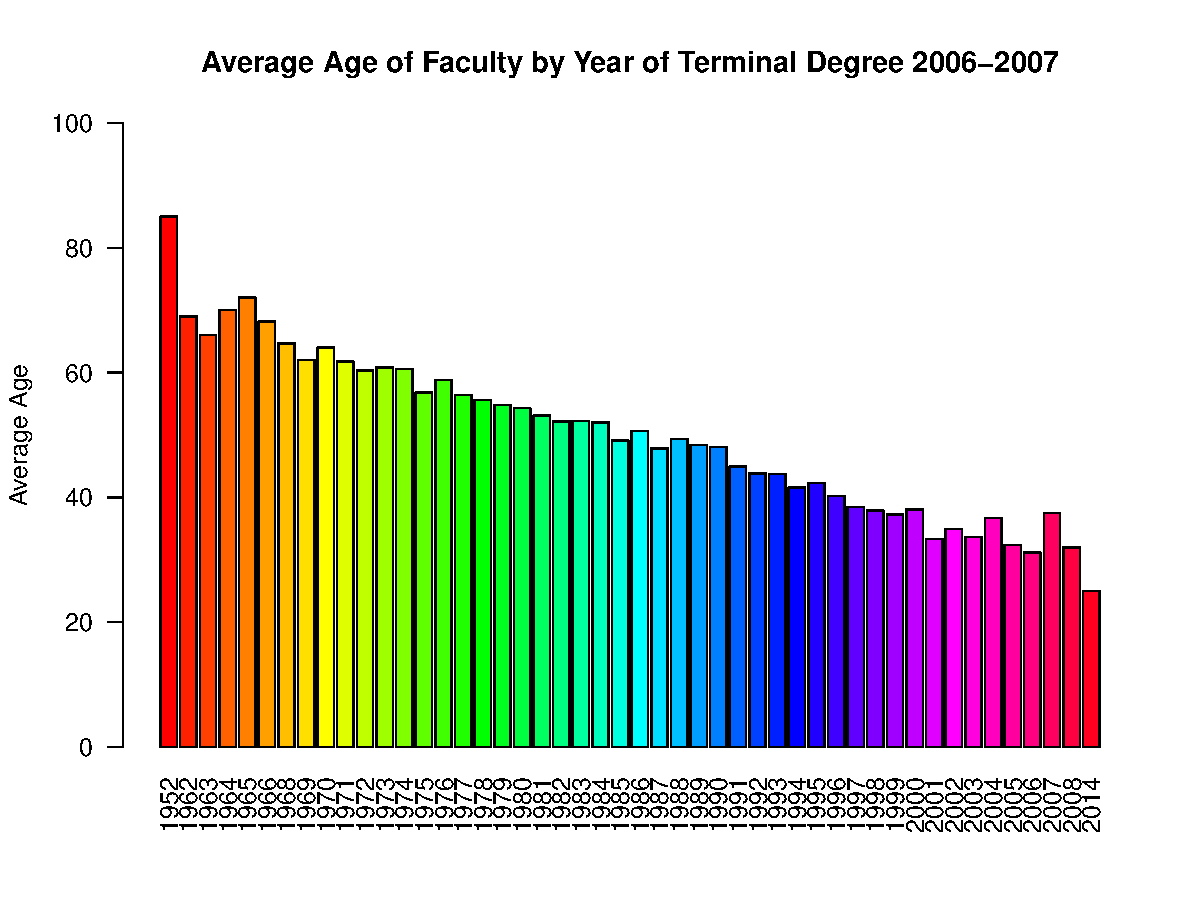
\includegraphics[width=\maxwidth]{figure/unnamed-chunk-12-3} 

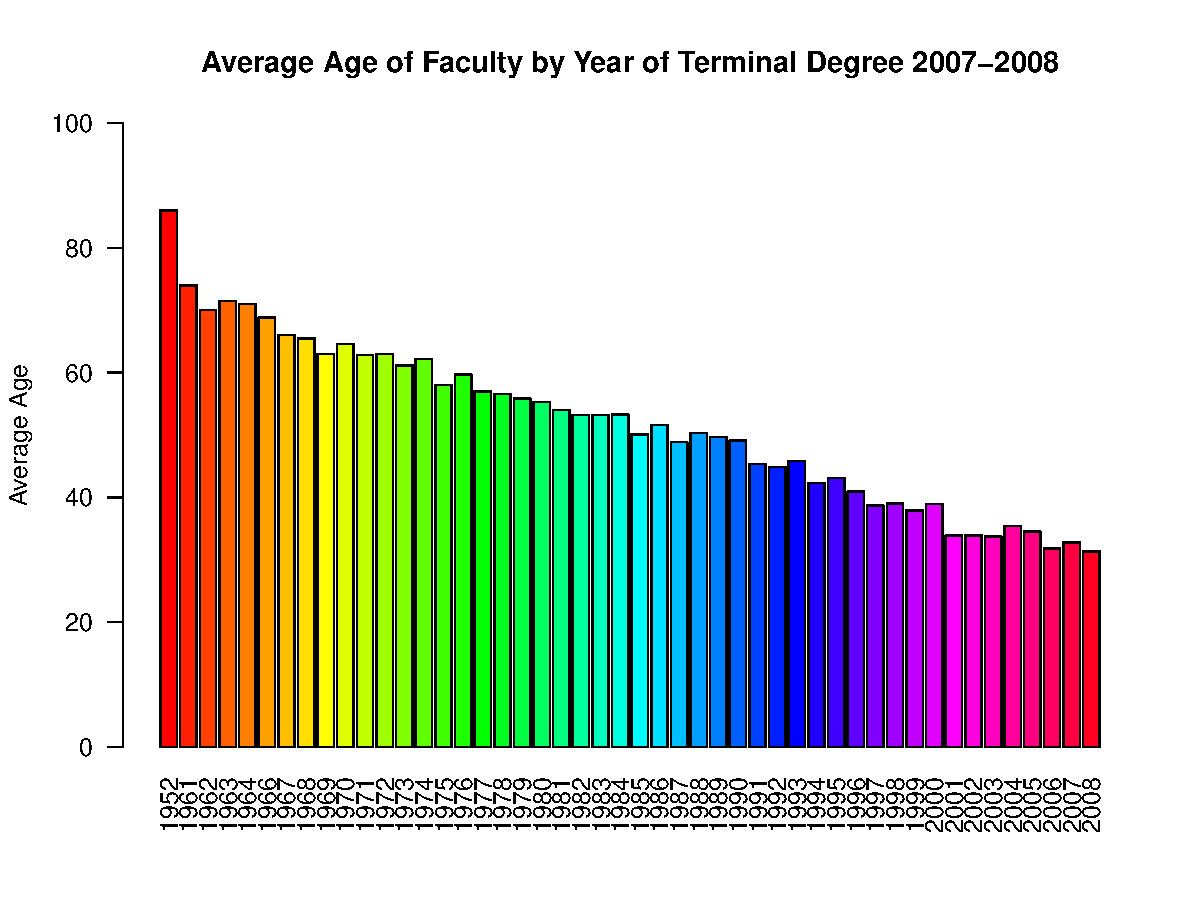
\includegraphics[width=\maxwidth]{figure/unnamed-chunk-12-4} 

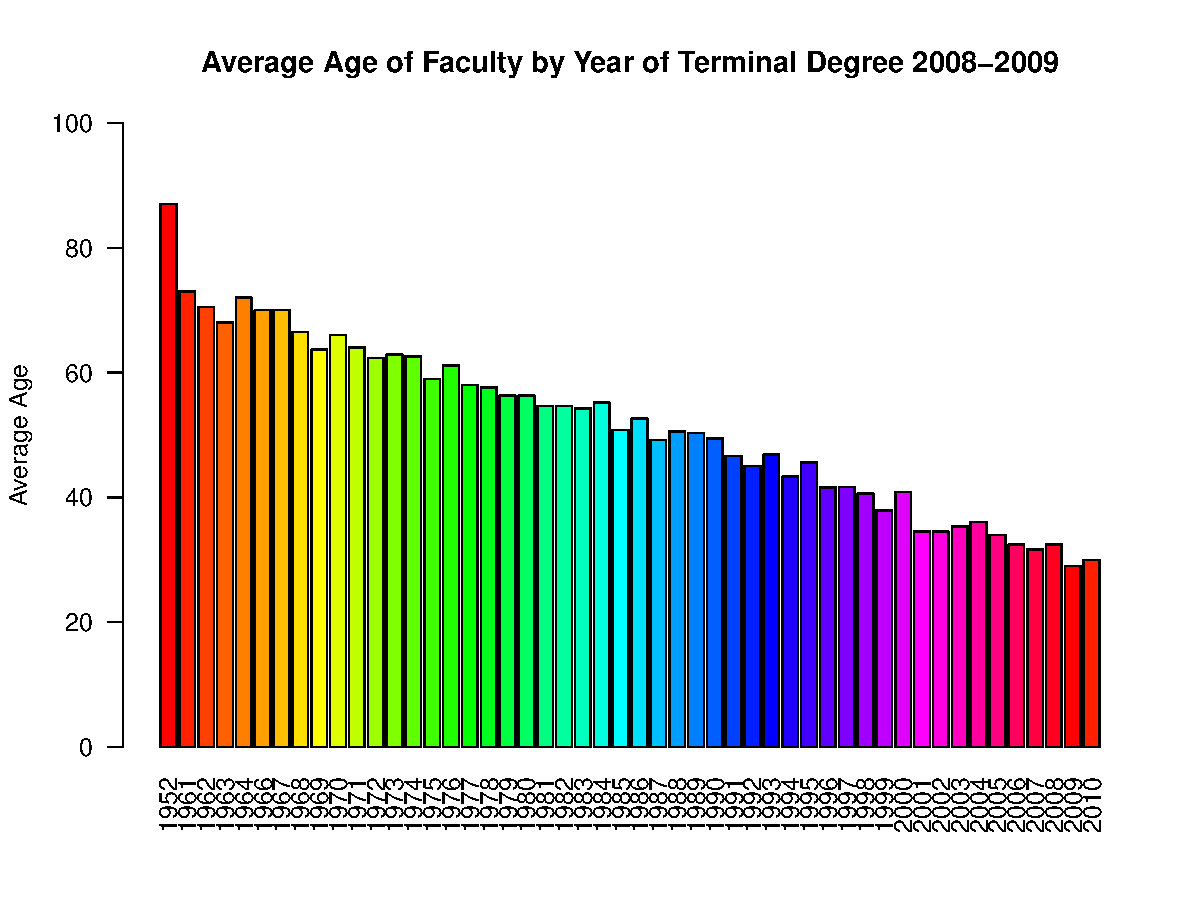
\includegraphics[width=\maxwidth]{figure/unnamed-chunk-12-5} 

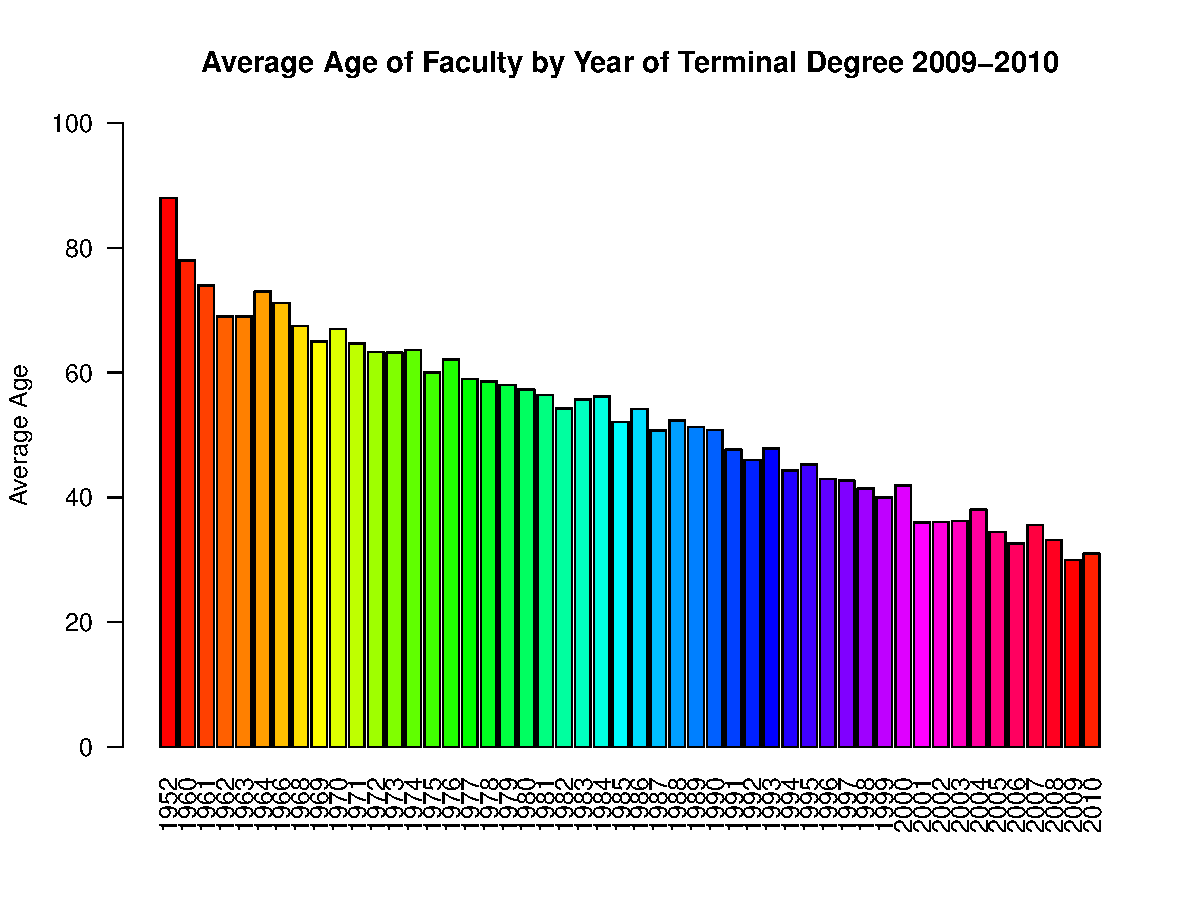
\includegraphics[width=\maxwidth]{figure/unnamed-chunk-12-6} 

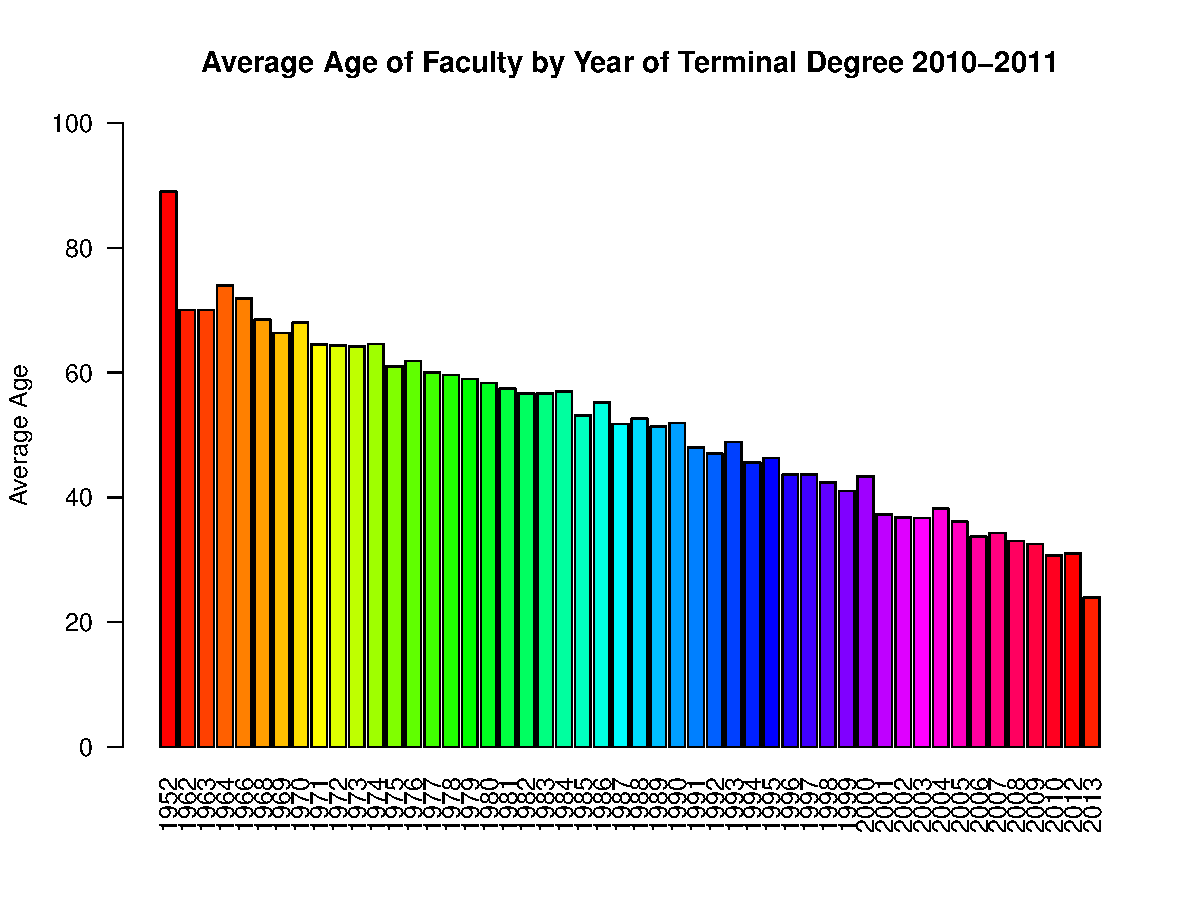
\includegraphics[width=\maxwidth]{figure/unnamed-chunk-12-7} 

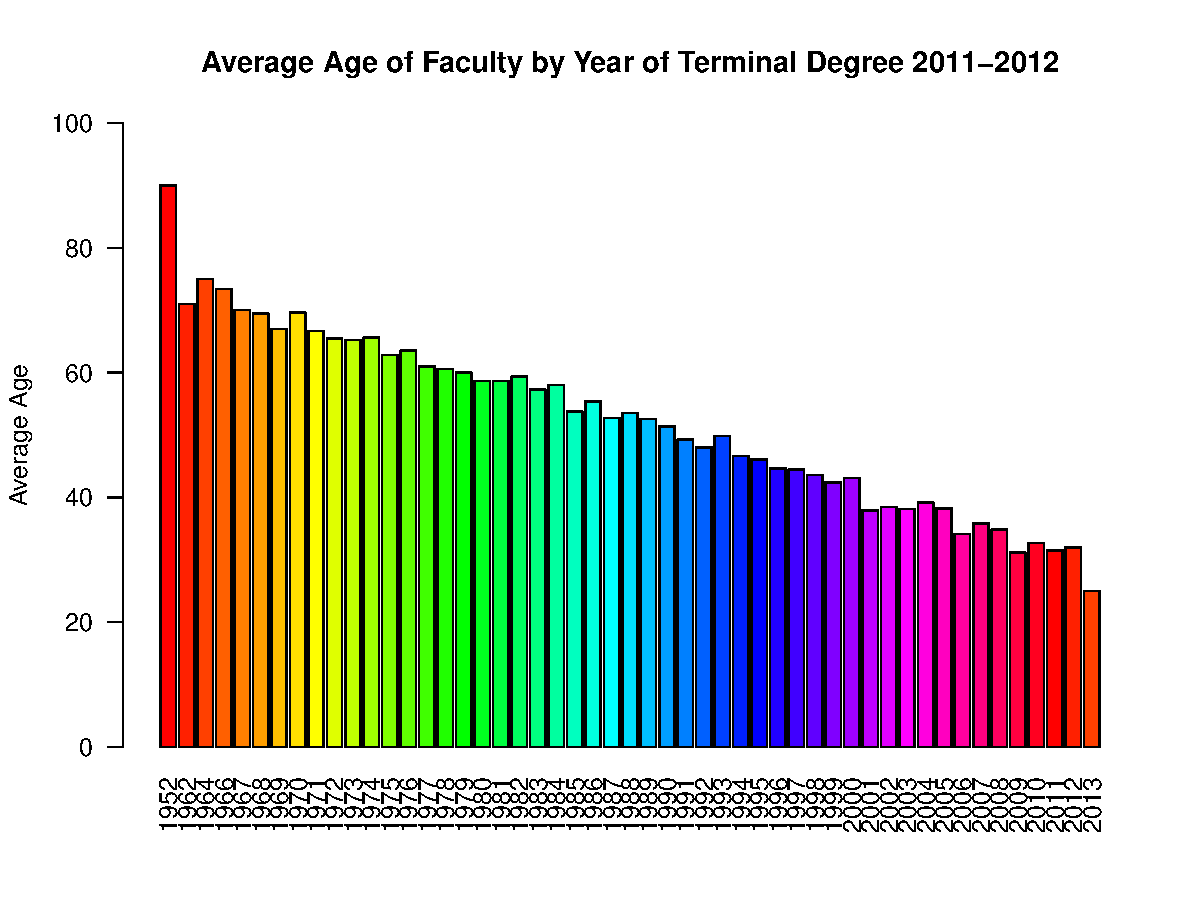
\includegraphics[width=\maxwidth]{figure/unnamed-chunk-12-8} 

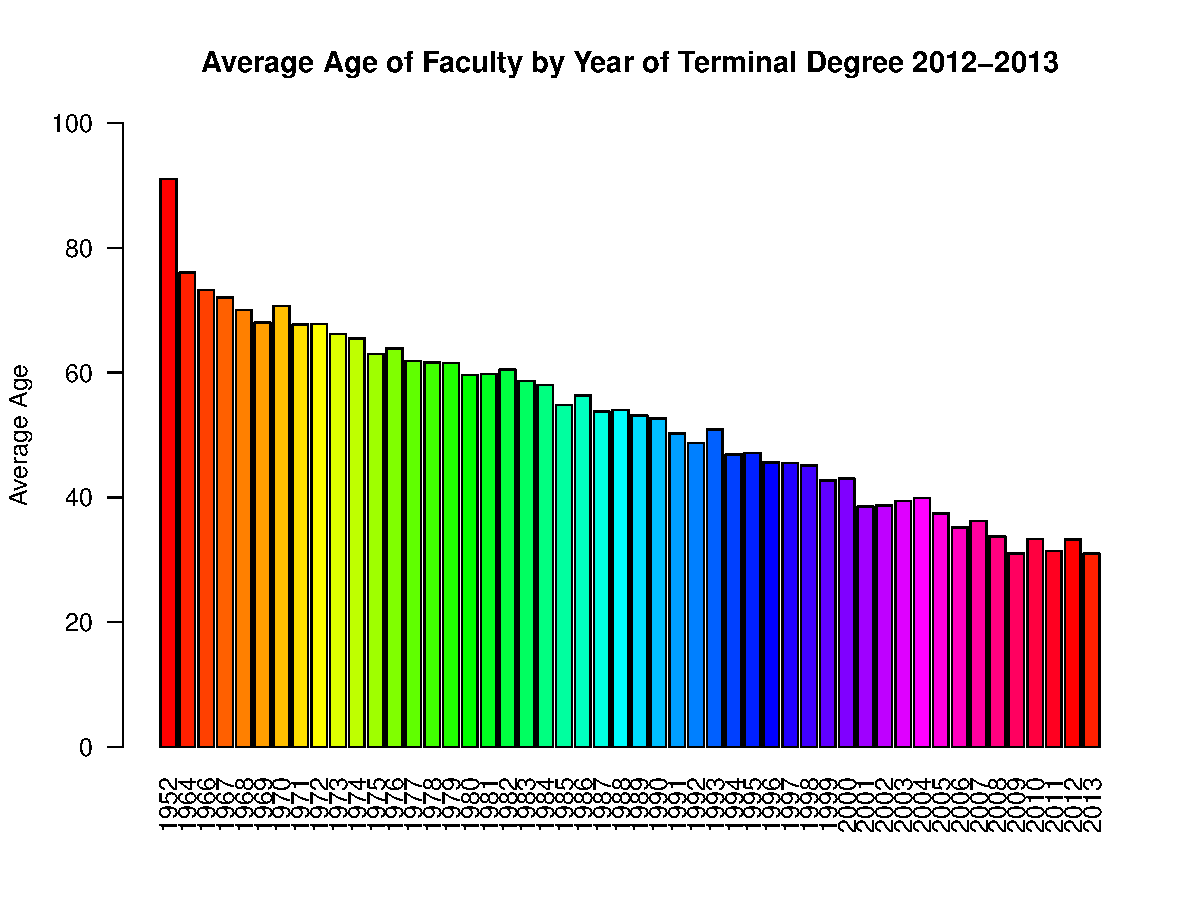
\includegraphics[width=\maxwidth]{figure/unnamed-chunk-12-9} 

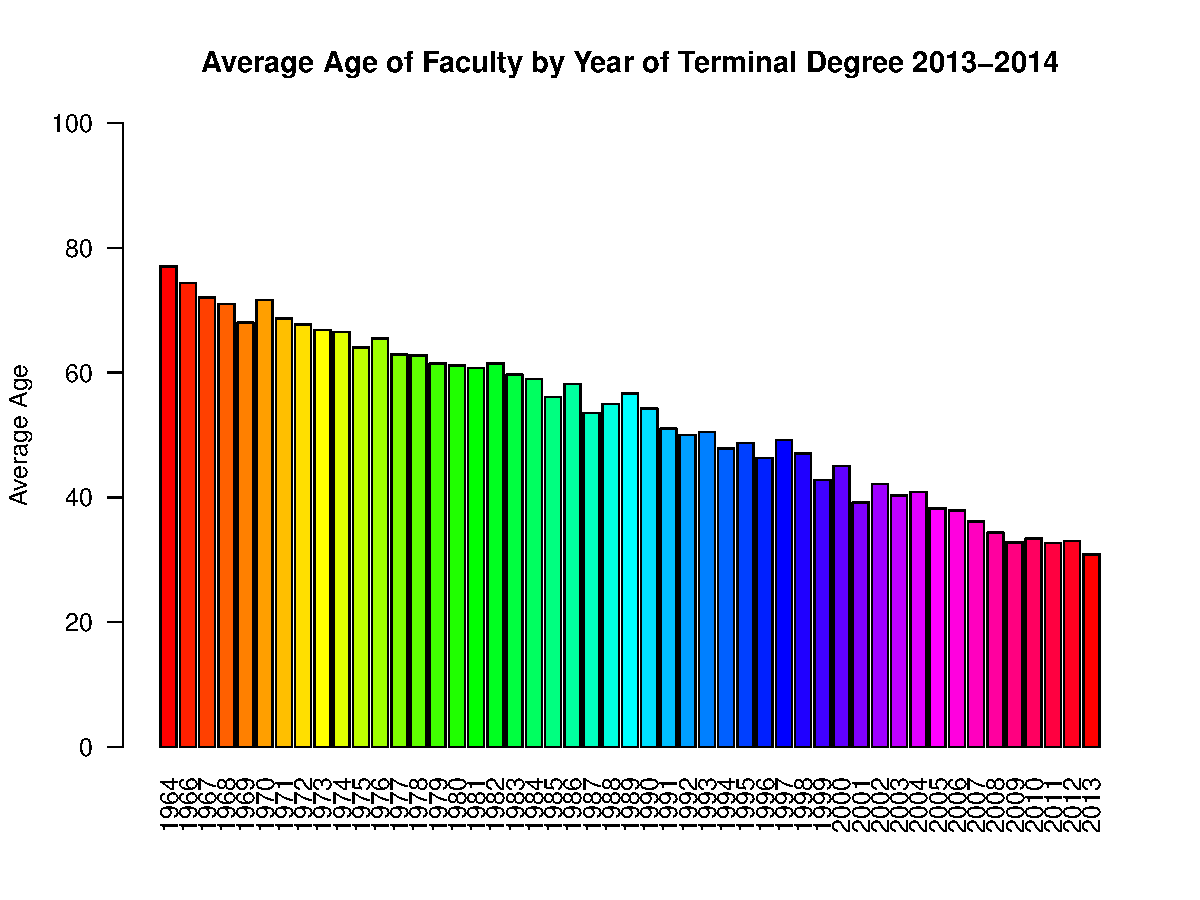
\includegraphics[width=\maxwidth]{figure/unnamed-chunk-12-10} 

\end{knitrout}

\bigskip
Do certain departments require more time to earn a PhD in than others?

\begin{knitrout}
\definecolor{shadecolor}{rgb}{0.969, 0.969, 0.969}\color{fgcolor}
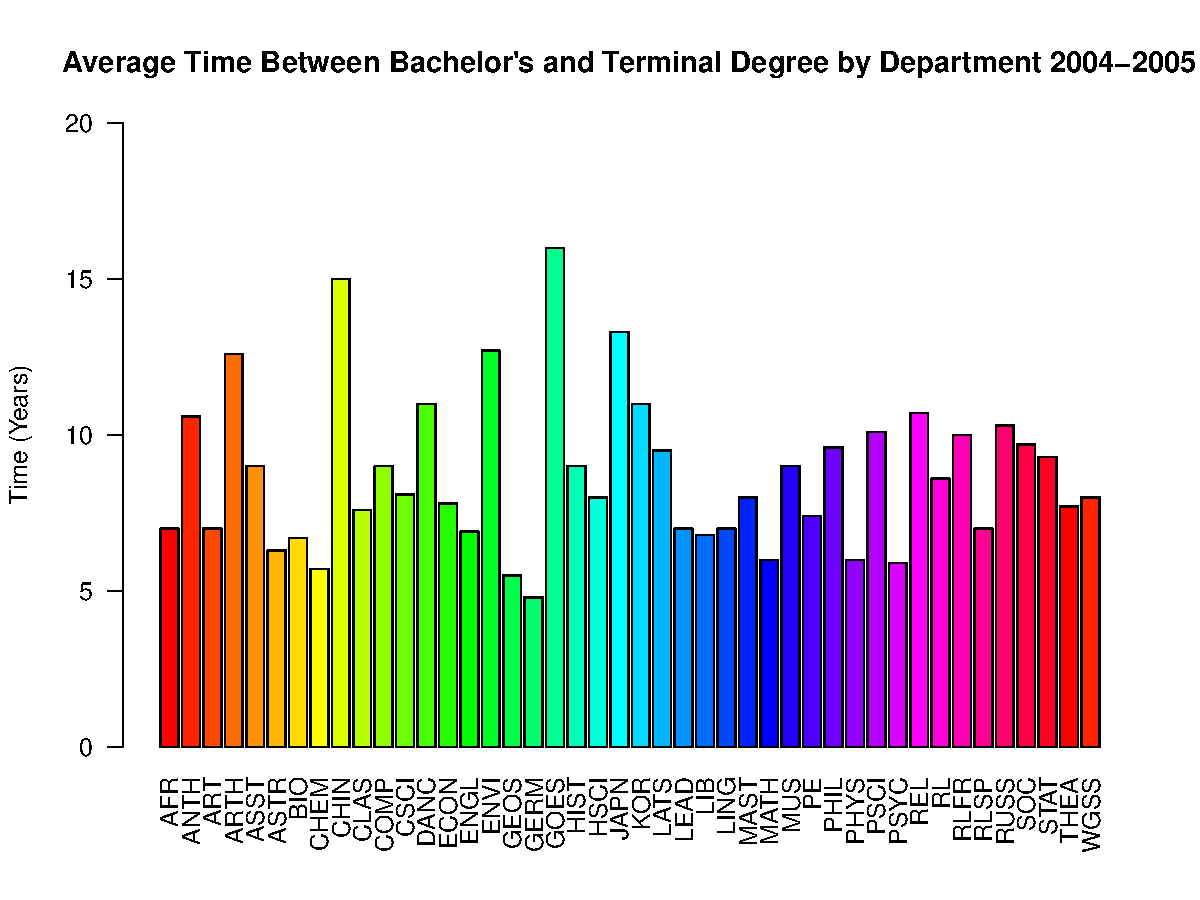
\includegraphics[width=\maxwidth]{figure/unnamed-chunk-13-1} 

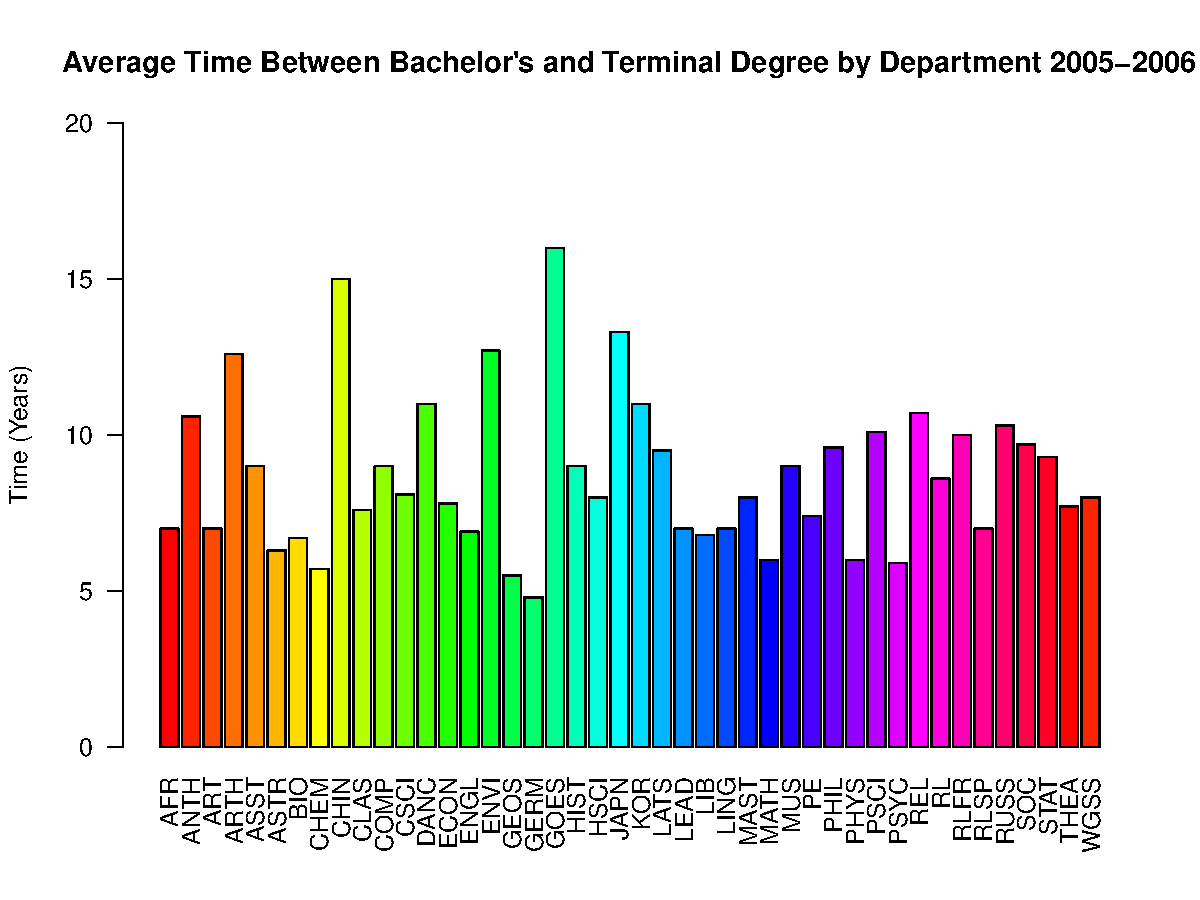
\includegraphics[width=\maxwidth]{figure/unnamed-chunk-13-2} 

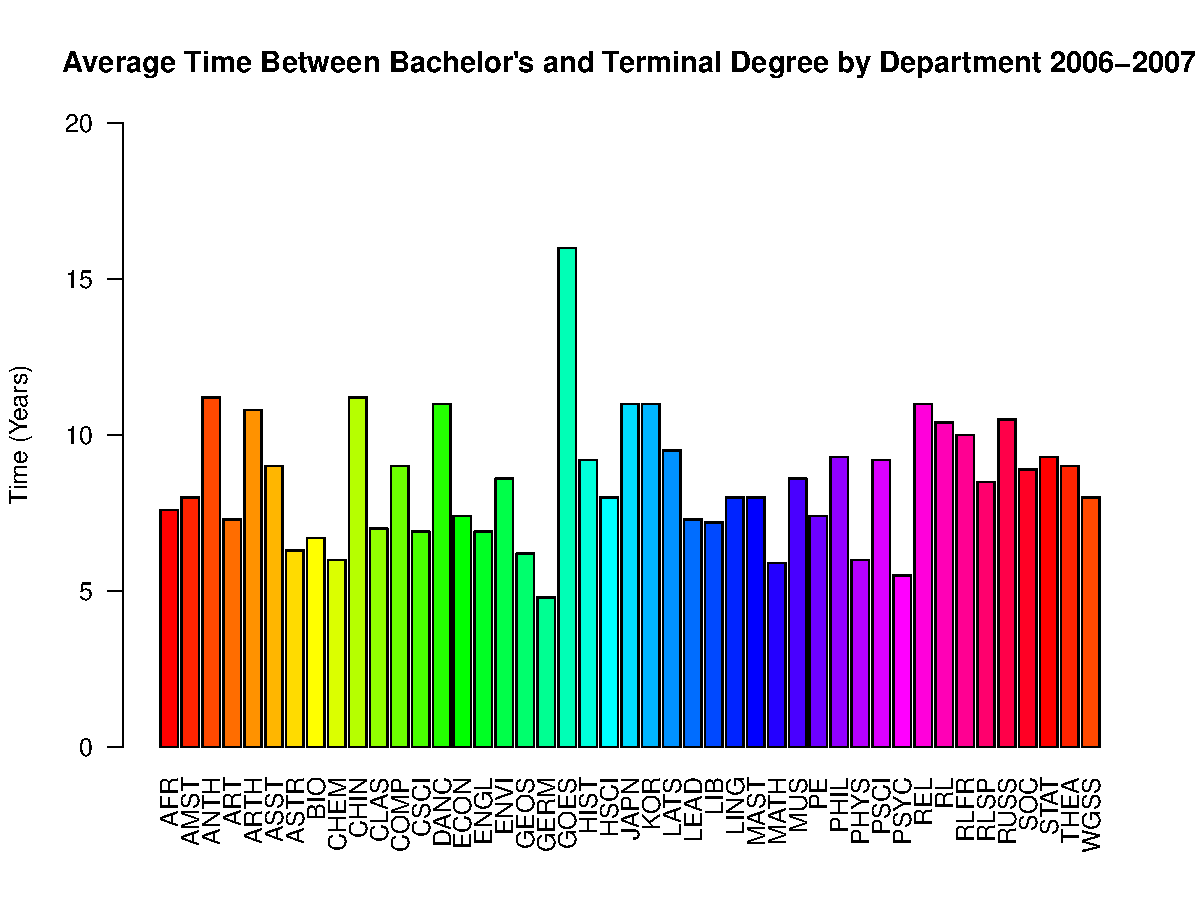
\includegraphics[width=\maxwidth]{figure/unnamed-chunk-13-3} 

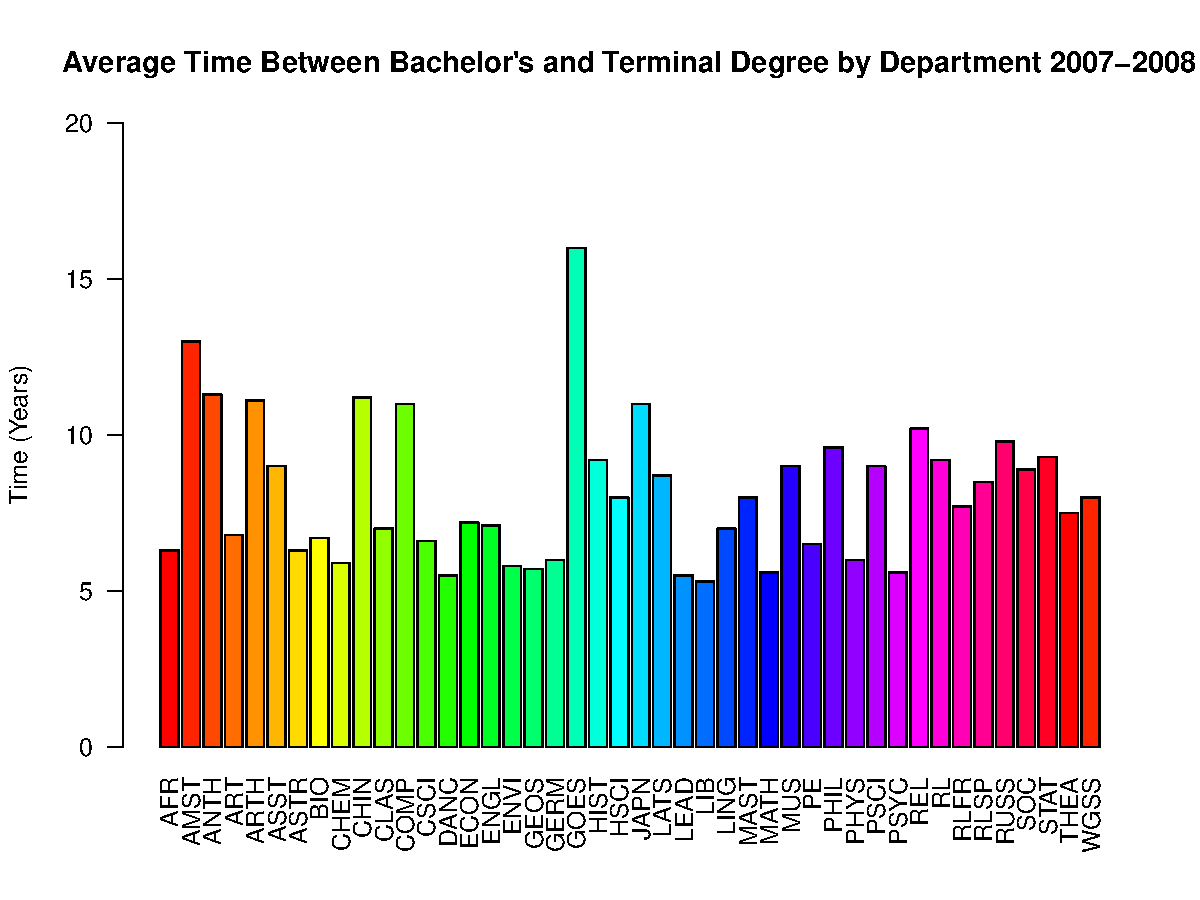
\includegraphics[width=\maxwidth]{figure/unnamed-chunk-13-4} 

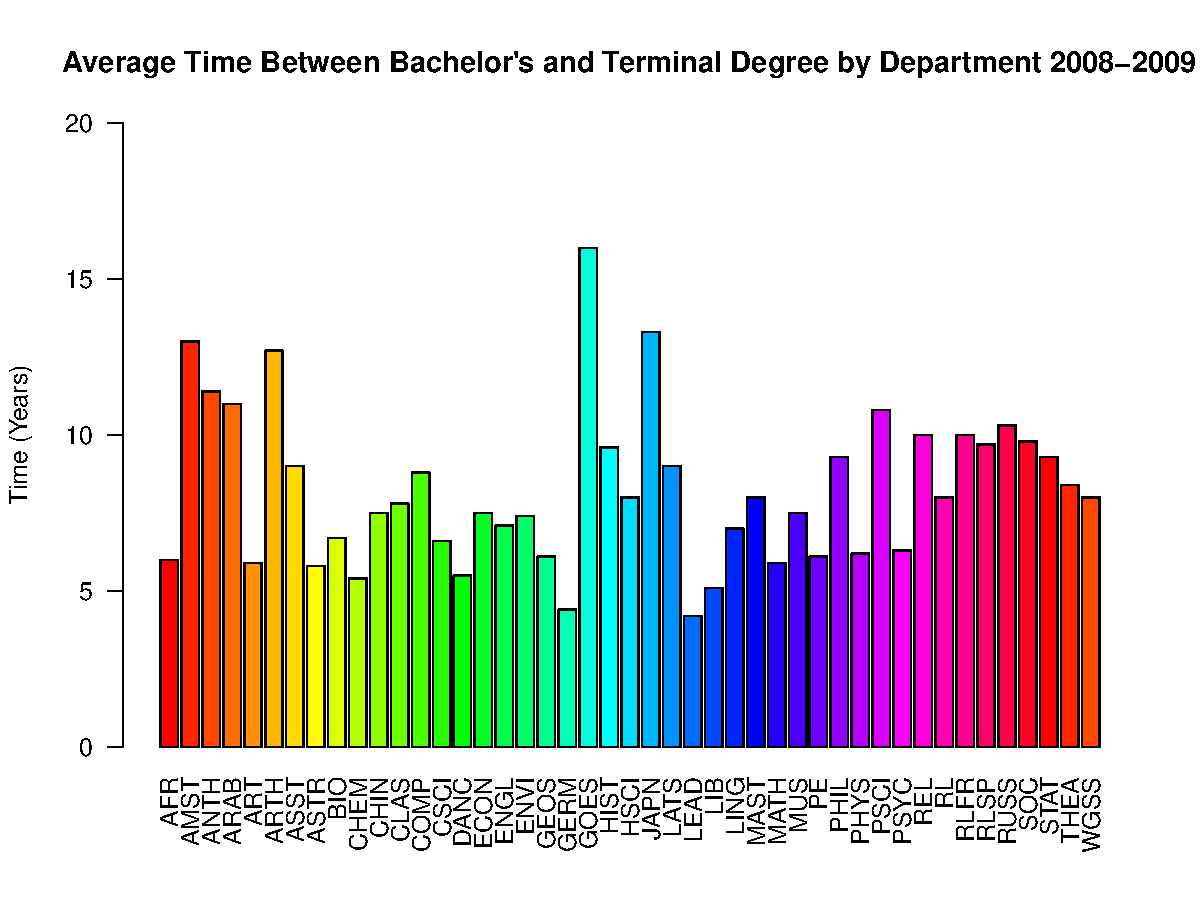
\includegraphics[width=\maxwidth]{figure/unnamed-chunk-13-5} 

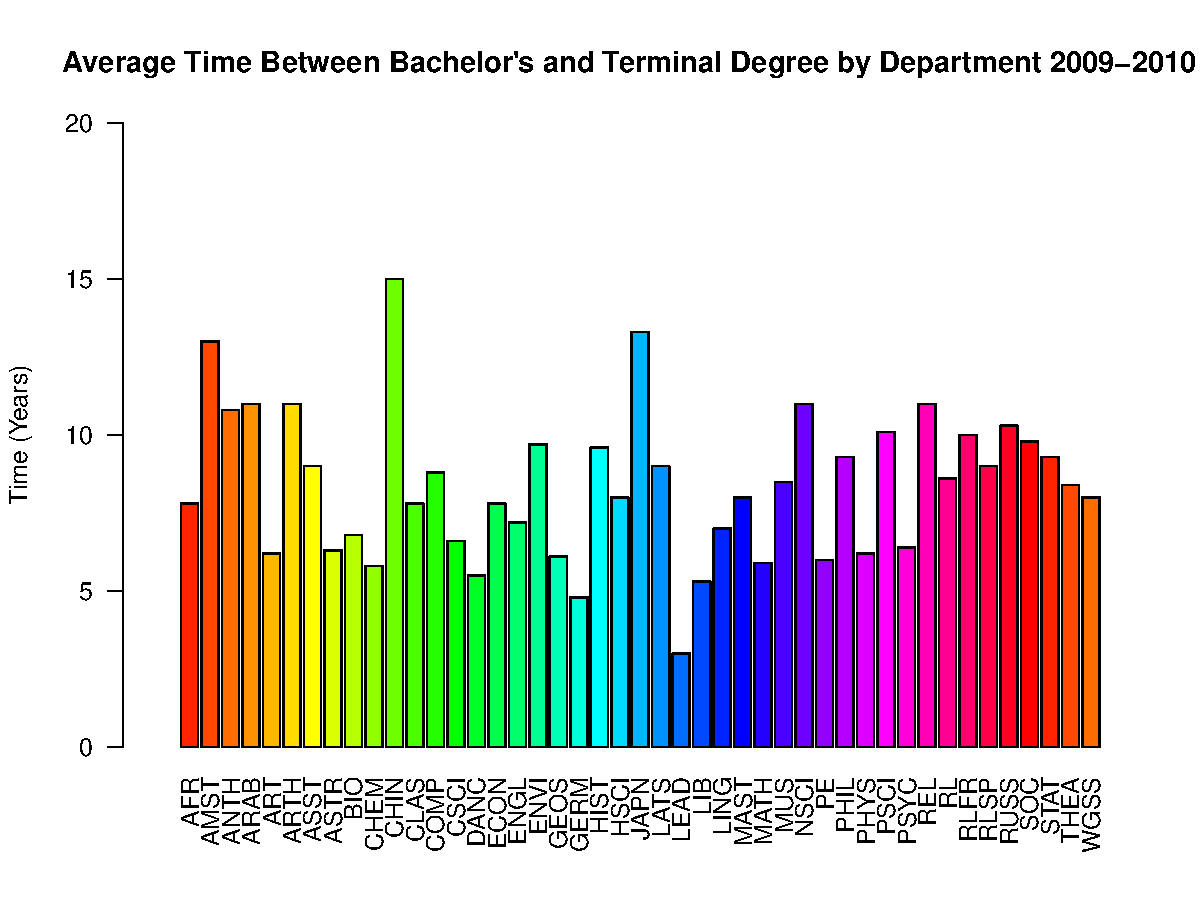
\includegraphics[width=\maxwidth]{figure/unnamed-chunk-13-6} 

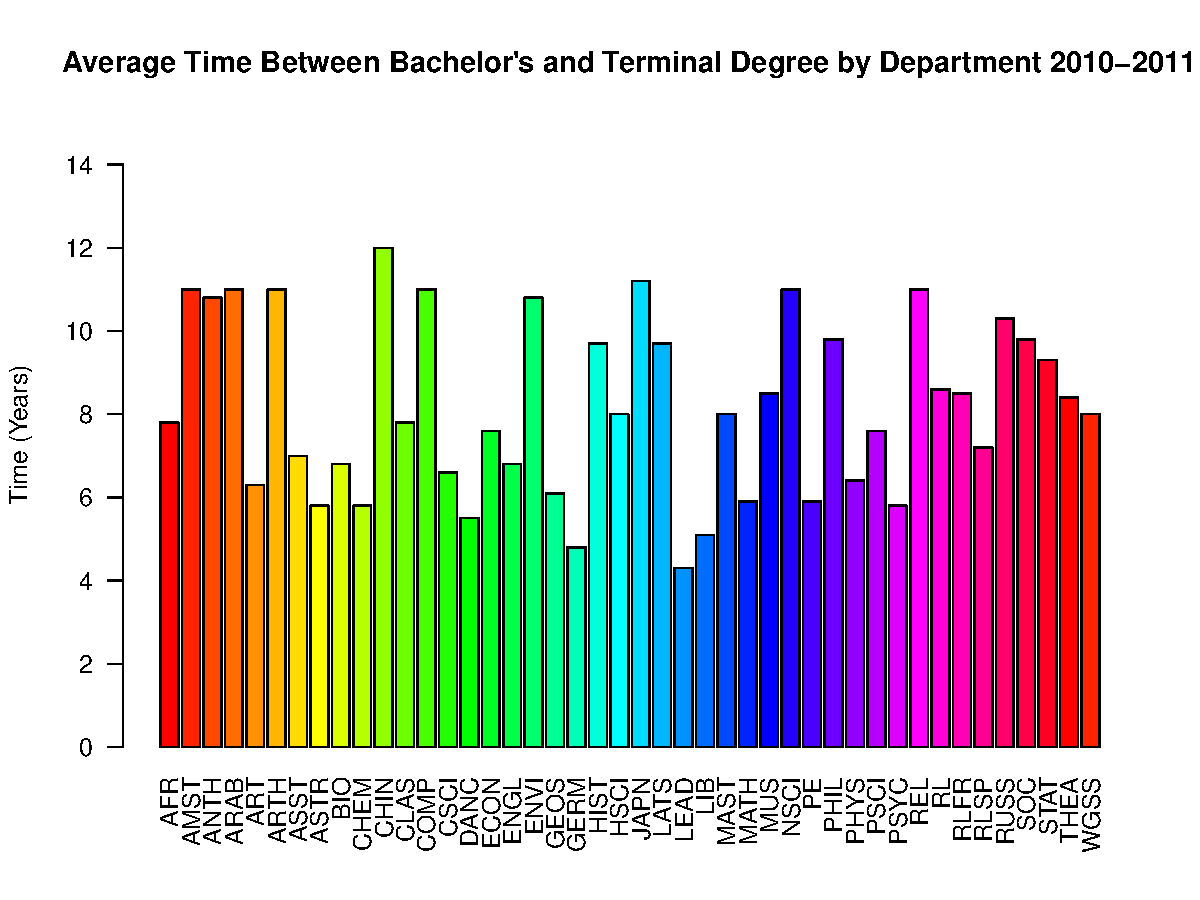
\includegraphics[width=\maxwidth]{figure/unnamed-chunk-13-7} 

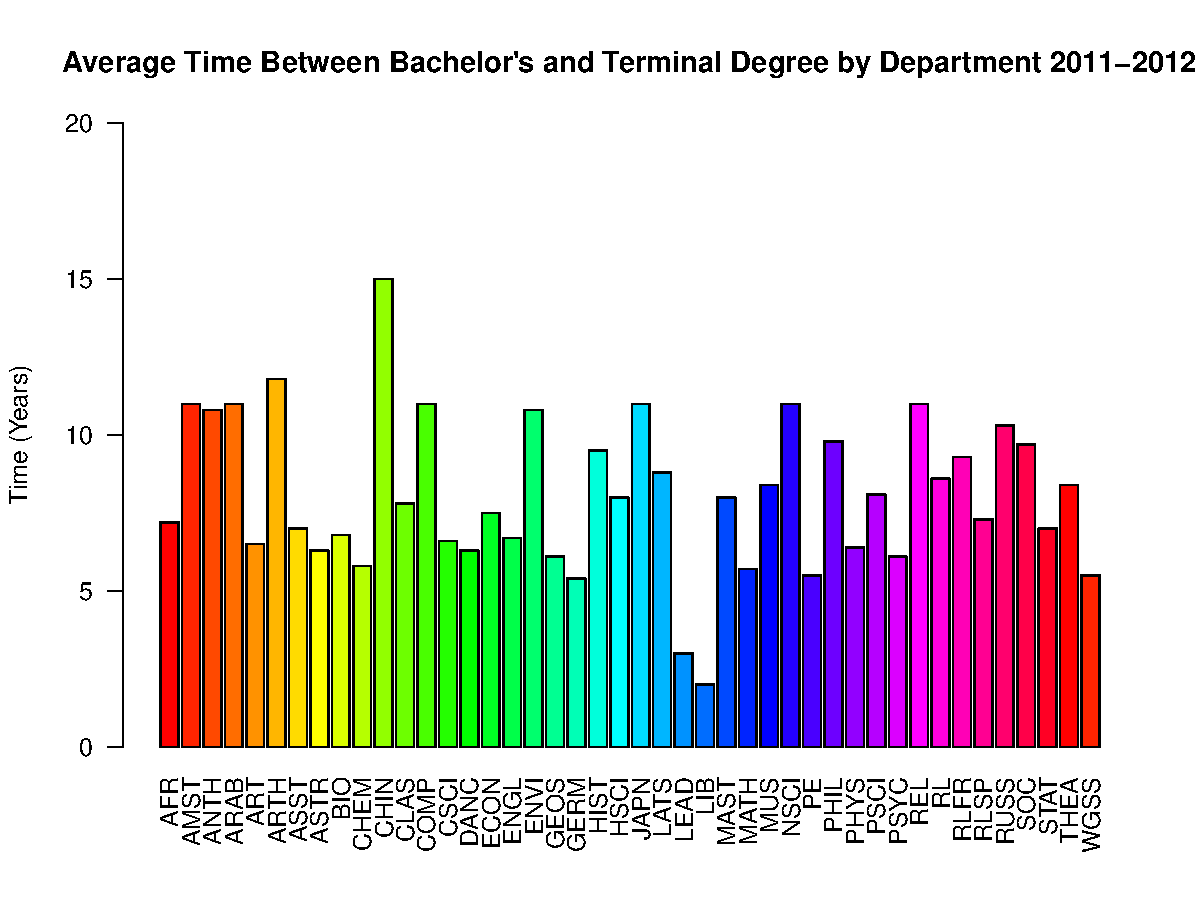
\includegraphics[width=\maxwidth]{figure/unnamed-chunk-13-8} 

\includegraphics[width=\maxwidth]{figure/unnamed-chunk-13-9} 

\includegraphics[width=\maxwidth]{figure/unnamed-chunk-13-10} 

\end{knitrout}

\bigskip
Has the actual, non bin Distribution of Ages changed significantly over the last 10 years with summary stats:

\begin{knitrout}
\definecolor{shadecolor}{rgb}{0.969, 0.969, 0.969}\color{fgcolor}
\includegraphics[width=\maxwidth]{figure/unnamed-chunk-14-1} 

\end{knitrout}

\begin{knitrout}
\definecolor{shadecolor}{rgb}{0.969, 0.969, 0.969}\color{fgcolor}\begin{kframe}
\begin{verbatim}
##    Min. 1st Qu.  Median    Mean 3rd Qu.    Max. 
##   24.00   36.00   45.00   45.07   53.00   83.00
\end{verbatim}
\end{kframe}
\end{knitrout}

\begin{knitrout}
\definecolor{shadecolor}{rgb}{0.969, 0.969, 0.969}\color{fgcolor}
\includegraphics[width=\maxwidth]{figure/unnamed-chunk-16-1} 

\end{knitrout}

\begin{knitrout}
\definecolor{shadecolor}{rgb}{0.969, 0.969, 0.969}\color{fgcolor}\begin{kframe}
\begin{verbatim}
##    Min. 1st Qu.  Median    Mean 3rd Qu.    Max. 
##   25.00   37.00   46.00   46.03   54.00   84.00
\end{verbatim}
\end{kframe}
\end{knitrout}


\begin{knitrout}
\definecolor{shadecolor}{rgb}{0.969, 0.969, 0.969}\color{fgcolor}
\includegraphics[width=\maxwidth]{figure/unnamed-chunk-18-1} 

\end{knitrout}

\begin{knitrout}
\definecolor{shadecolor}{rgb}{0.969, 0.969, 0.969}\color{fgcolor}\begin{kframe}
\begin{verbatim}
##    Min. 1st Qu.  Median    Mean 3rd Qu.    Max. 
##   25.00   36.00   45.00   45.75   54.00   85.00
\end{verbatim}
\end{kframe}
\end{knitrout}

\begin{knitrout}
\definecolor{shadecolor}{rgb}{0.969, 0.969, 0.969}\color{fgcolor}
\includegraphics[width=\maxwidth]{figure/unnamed-chunk-20-1} 

\end{knitrout}

\begin{knitrout}
\definecolor{shadecolor}{rgb}{0.969, 0.969, 0.969}\color{fgcolor}\begin{kframe}
\begin{verbatim}
##    Min. 1st Qu.  Median    Mean 3rd Qu.    Max. 
##   27.00   37.00   46.00   46.53   55.00   86.00
\end{verbatim}
\end{kframe}
\end{knitrout}


\begin{knitrout}
\definecolor{shadecolor}{rgb}{0.969, 0.969, 0.969}\color{fgcolor}
\includegraphics[width=\maxwidth]{figure/unnamed-chunk-22-1} 

\end{knitrout}

\begin{knitrout}
\definecolor{shadecolor}{rgb}{0.969, 0.969, 0.969}\color{fgcolor}\begin{kframe}
\begin{verbatim}
##    Min. 1st Qu.  Median    Mean 3rd Qu.    Max. 
##   23.00   37.00   47.00   46.99   56.00   87.00
\end{verbatim}
\end{kframe}
\end{knitrout}

\begin{knitrout}
\definecolor{shadecolor}{rgb}{0.969, 0.969, 0.969}\color{fgcolor}
\includegraphics[width=\maxwidth]{figure/unnamed-chunk-24-1} 

\end{knitrout}

\begin{knitrout}
\definecolor{shadecolor}{rgb}{0.969, 0.969, 0.969}\color{fgcolor}\begin{kframe}
\begin{verbatim}
##    Min. 1st Qu.  Median    Mean 3rd Qu.    Max. 
##   26.00   39.00   48.00   48.32   57.00   88.00
\end{verbatim}
\end{kframe}
\end{knitrout}


\begin{knitrout}
\definecolor{shadecolor}{rgb}{0.969, 0.969, 0.969}\color{fgcolor}
\includegraphics[width=\maxwidth]{figure/unnamed-chunk-26-1} 

\end{knitrout}

\begin{knitrout}
\definecolor{shadecolor}{rgb}{0.969, 0.969, 0.969}\color{fgcolor}\begin{kframe}
\begin{verbatim}
##    Min. 1st Qu.  Median    Mean 3rd Qu.    Max. 
##   24.00   39.00   48.50   48.67   58.00   89.00
\end{verbatim}
\end{kframe}
\end{knitrout}

\begin{knitrout}
\definecolor{shadecolor}{rgb}{0.969, 0.969, 0.969}\color{fgcolor}
\includegraphics[width=\maxwidth]{figure/unnamed-chunk-28-1} 

\end{knitrout}

\begin{knitrout}
\definecolor{shadecolor}{rgb}{0.969, 0.969, 0.969}\color{fgcolor}\begin{kframe}
\begin{verbatim}
##    Min. 1st Qu.  Median    Mean 3rd Qu.    Max. 
##   25.00   39.00   48.00   48.72   58.00   90.00
\end{verbatim}
\end{kframe}
\end{knitrout}



\begin{knitrout}
\definecolor{shadecolor}{rgb}{0.969, 0.969, 0.969}\color{fgcolor}
\includegraphics[width=\maxwidth]{figure/unnamed-chunk-30-1} 

\end{knitrout}

\begin{knitrout}
\definecolor{shadecolor}{rgb}{0.969, 0.969, 0.969}\color{fgcolor}\begin{kframe}
\begin{verbatim}
##    Min. 1st Qu.  Median    Mean 3rd Qu.    Max. 
##   24.00   38.00   47.50   48.19   58.00   91.00
\end{verbatim}
\end{kframe}
\end{knitrout}

\begin{knitrout}
\definecolor{shadecolor}{rgb}{0.969, 0.969, 0.969}\color{fgcolor}
\includegraphics[width=\maxwidth]{figure/unnamed-chunk-32-1} 

\end{knitrout}

\begin{knitrout}
\definecolor{shadecolor}{rgb}{0.969, 0.969, 0.969}\color{fgcolor}\begin{kframe}
\begin{verbatim}
##    Min. 1st Qu.  Median    Mean 3rd Qu.    Max. 
##   24.00   38.00   47.00   48.08   58.00   77.00
\end{verbatim}
\end{kframe}
\end{knitrout}









\end{document}
